\documentclass[12pt, twoside]{report}
\usepackage{sectsty}
\usepackage[utf8]{inputenc}
\usepackage[croatian]{babel}
\usepackage{graphicx}

\graphicspath{ {Images/} }
%\usepackage{lipsum}
\usepackage[a4paper,width=150mm,top=25mm,bottom=25mm,bindingoffset=6mm]{geometry}
\usepackage{fancyhdr}
\usepackage{xcolor}
\usepackage{tcolorbox}
%\usepackage{draftwatermark}
\usepackage{amsmath,tabstackengine}
\usepackage[section]{placeins}
\usepackage{tikz}
\usepackage{textcomp}
\usepackage[OT1]{fontenc}
\usepackage[utf8]{inputenc}
\usepackage{lmodern}
\usepackage{csquotes}
\usepackage[framed,numbered,autolinebreaks,useliterate]{mcode}
\usetikzlibrary{shapes,arrows,positioning,calc}


\pagestyle{fancy}
\fancyhead{}
\fancyhead[RO,LE]{Proporcionalna navigacija i upravljanje kretanja projektila}
\setlength{\headheight}{15pt}
\fancyfoot{}
\fancyfoot[CO,RE]{\thepage}
\renewcommand{\headrulewidth}{0.4pt}
\renewcommand{\footrulewidth}{0.4pt}


%\SetWatermarkText{Nedovršeno}
%\SetWatermarkScale{1}
% https://en.wikibooks.org/wiki/LaTeX/Floats,_Figures_and_Captions
\usepackage{caption}
\usepackage{subcaption}

% References
\usepackage[style=authoryear,sorting=ynt]{biblatex}
\addbibresource{references.bib}

% https://en.wikibooks.org/wiki/LaTeX/Text_Formatting#Line_Spacing
\usepackage{setspace}
\singlespacing
\onehalfspacing
%\doublespacing
%\setstretch{1.1}
\hbadness=99999
\usepackage{titlesec,blindtext,color}

\definecolor{gray75}{gray}{0.75}
\newcommand{\hsp}{\hspace{20pt}}
\titleformat{\chapter}[hang]{\Huge\bfseries}{}{0pt}{\Huge\bfseries}
\begin{document}
\tikzset{
block/.style = {draw, fill=white, rectangle, minimum height=3em, minimum width=3em},
tmp/.style  = {coordinate}, 
sum/.style= {draw, fill=white, circle, node distance=1cm},
input/.style = {coordinate},
output/.style= {coordinate},
pinstyle/.style = {pin edge={to-,thin,black}
}
}
\begin{titlepage}
    \begin{center}
        \vspace*{1cm}
        
        \Huge
        \textbf{Navigacija i upravljanje projektila}
        
        %\vspace{0.5cm}
        
       % \LARGE
        %Thesis Subtitle
        
        \vspace{1.5cm}
        
        \Large
        \textbf{Mirza Hodžic}\\
        
        \vspace{0.5cm}
        
        Mentor: prof. dr. Naser Prljača\\
        
        \vfill
        
        
\includegraphics[width=0.5\textwidth]{Images/preuzmi.png}
        
        \vspace{0.8cm}
        
        \Large
        A thesis presented for the degree of Doctor of Philosophy
        
        \vspace{0.5cm}
        
        \LARGE
	    \textsc{Fakultet eleketrotehnike\\
	    Univerzitet u Tuzli}
	    
	    \begin{flushright}
	
	    \Large
	    Date
	
	    \end{flushright}
        
    \end{center}
\end{titlepage}

\chapter*{Posveta}
Mojim roditeljima

%\chapter*{Declaration}
%I declare that..

%\chapter*{Acknowledgements}
%I want to thank...
\tableofcontents

%\listoffigures
%\listoftables
\newpage
\thispagestyle{plain}
\begin{center}
    \Large
    \textbf{Thesis Title}
    
    \vspace{0.4cm}
    \large
    Thesis Subtitle
    
    \vspace{0.4cm}
    \textbf{Author Name}
    
    \vspace{0.9cm}
    \textbf{Abstract}
\end{center}

\lipsum[1-3]

%\chapter[]{Uvod}
%\input{Chapters/introduction}

\chapter{Jednačine kretanja tijela}
\section{Koordinatni sistemi}
Orijentacija osa koordinatnog sistema preko kojih su određeni 
vektori ili tenzori potpuno je proizvoljna. Obično se jedna od osi(e.g. $x$ osa) poravnava 
sa geometrijskom osom tijela. 
Ako se tijelo kreće stalnom brzinom tada se jedan koordinatni sistem može 
koristiti za sve veličine, međutim ako se tijelo rotira tada se naslućuju dva koordinatna sistema:
\begin{itemize}
    \item Koordinatni sistem vezan za zemlju
    \item Koordinatni sistem vezan za tijelo
\end{itemize}
Koordinatni sistem vezan za zemlju je inertcijalni iako se zemlje rotira u odnosu na geomtrijsku osu.
Sastoji se od tri ordinate, jedna predstavlja poziciju po sjevernoj osi, jedna po lokaloj istočnoj osi 
i jedna predstavlja vertikalnu poziciju. Ose koordinatnog sistema vezanog za zemlju su 
označene sa $X_e, Y_e, Z_e$. Drugim riječima, $X_e$ i $Y_e$ leže u ravni dok je $Z_e$ usmjeren ka centru Zemlje.\\
Koordinatni sistem vezan za tijelo sastoji se iz tri ordinate sa ishodištem u centru gravitacije letjelice: $x$ osa koja je
usmjerena ka nosu letjelice tj. podudara se sa longitudinalnom osom, $y$ ose koja je usmjerena ka desnom krilu letjelice i $z$ ose koja dopunjava lijevo orijentisani 
koordinatni sistem.
\begin{figure}[!ht]
    \centering
    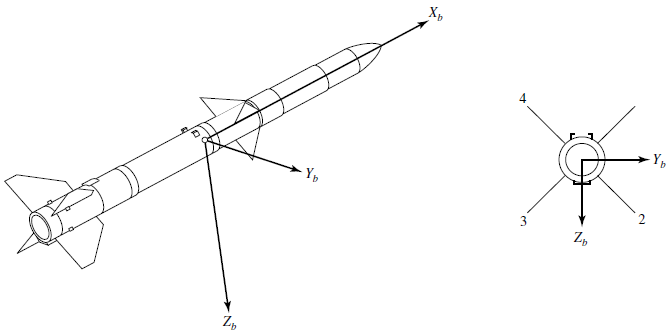
\includegraphics[scale=0.7]{body.png}
    \caption{Koordinatni sistem vezan za tijelo}
    \label{fig:KBS}
\end{figure}
Da se definiše položaj letjelice u odnosu na koordinatni sistem koriste se Eulerovi uglovi($\psi, \theta, \phi$).
\begin{figure}[!ht]
    \centering
    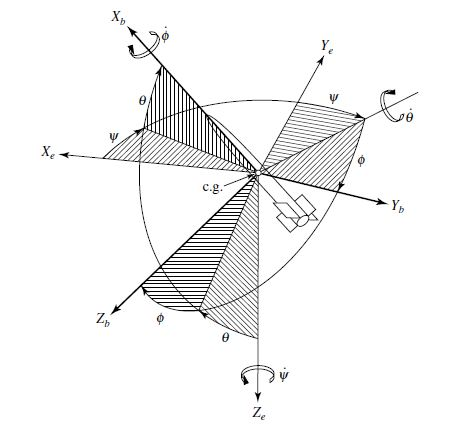
\includegraphics[scale=0.7]{earth-body.JPG}
    \caption{Eulerovi uglovi}
\end{figure}
Ovo znači da se bilo koja rotacija, odnosno transformacija iz sistema tijela u sistem Zemlje može postići sa tri rotacije oko osi i to prva 
rotacija za ugao $\phi$ oko longitudinalne, za ugao $\theta$ oko lateralne i za ugao 
$\psi$ oko normalne ose. Transformacija $T_b^e$ koja ostvaruje transformaciju iz 
koordinatnog sistema vezanog za zemlju u koordinatni sistem vezan za tijelo je data sa:
\begin{equation}
    T_{z \to b} = T_1(\phi)T_2(\theta)T_3(\psi)
\end{equation}
,gdje je:
\begin{align}
    T_1(\phi) =& \begin{bmatrix}
        1 & 0 & 0\\
        0 & \cos\phi & \sin\phi \\
        0 & -\sin\phi & \cos\phi 
    \end{bmatrix}\\
     T_2(\theta)=& \begin{bmatrix}
        \cos\theta & 0 & -\sin\theta \\
         0 & 1 & 0\\
         \sin\theta & 0 & \cos\theta
    \end{bmatrix}\\
    T_3(\psi) = &\begin{bmatrix}
        \cos\psi & \sin\phi & 0\\
        -\sin\phi & \cos\phi & 0\\
        0 & 0 & 1
    \end{bmatrix}
\end{align}
,odnosno:
\begin{equation}
    {\footnotesize
    T_{z \to b}=\begin{bmatrix}
        cos\theta cos\psi && cos\theta sin\psi && -sin\theta\\
        sin\phi sin\theta cos\psi-cos\phi sin\psi && sin\phi sin\theta sin\psi +cos\phi cos\psi&& sin\phi cos\theta\\
        c\phi s\theta c\psi+sin\phi sin\psi && cos\phi sin\theta sin\psi -sin\phi cos\psi&& cos\phi cos\theta\\
    \end{bmatrix}}
    \label{eq:ztob}
\end{equation}
Treba primjetiti da rezultantna matrica $T_{z \to b}$ može imati singularitete, pa se domen
Eulerovih uglova ograničava na sljedeći način:
\begin{align*}
    -\pi \leq \phi <\pi \quad ili \quad 0\leq\phi<2\pi \\
    -\pi \leq \psi <\pi \qquad \qquad \qquad \qquad \\
    -\frac{\pi}{2}\leq \theta \leq \frac{\pi}{2} \quad ili \quad 0\leq\psi<2\pi
\end{align*}
Ovo znači da u ovom slučaju postoji beskonačno mnogo načina da se ostvari željena transformacija.
Ovaj problem se može riješiti uvođenjem jediničnog kvaterniona.
Još jedan iznimno važan koordinatni sistem je \textit{koordinatni sistem brzine tijela(BKS)}. Ovaj Koordinatni
sistem se koristi kad god relativno kretanje objekta u odnosu na okolinu ima za posljedicu pojavu 
reaktivnih sila. Koordinatni sistem brzine je vezan za vektor brzinu objekta. Ishodište kooridnatnog sistema 
sitema brzine tijela se podudara sa centrom mase tijela(centar mase se može mijenjati tokom leta zbog utroška goriva), dok 
je $X$ osa kolinearna sa vektorom brzine objekta. Druge dvije ose se proizvoljno definišu u ravni 
normalnoj na vektor brzine. Najčešće se uzima da $Z$ osa zadovoljava barem jedan od naredna dva uslova:
\begin{itemize}
    \item $Z$ leži u presjeku ravni normalne na vektor brzine i vertikalne ravni simetrije pokretnog objekta.
    \item $Z$ leži u presjeku ravni normalne na vektor brzine i vertikalne ravni referentnog koordinatnog sistema.
\end{itemize}
Koordinatni sistem brzine je prikazan na slici \ref{fig:vks}.
\begin{figure}[!ht]
    \centering
    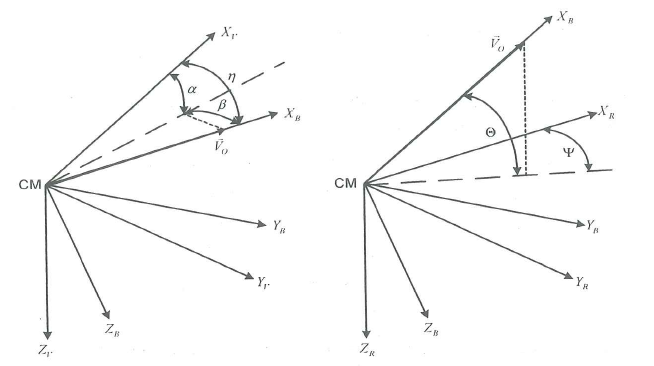
\includegraphics[scale=0.5]{vks.PNG}
    \caption{Ubacicu svoju sliku}
    \label{fig:vks}
\end{figure}
Ugao između $X$ ose sitema tijela i $X$ ose sitema brzine je označen sa $\eta$ i ovim uglom se i definiše 
koordinatni sistem brzine tijela. Ugao $\alpha$ je ugao ugao između $Z_b$ ose  sistema tijela i projekcije 
vektora brzine na vertikalnu ravan sistema tijela. Ovaj ugao se napadni ugao o kojem će više riječi biti kasnije. 
Ugao $\beta$ je ugao izmešu vektora brzine i vertikalne ravni sistema tijela. Ovaj ugao se zove ugao klizanja i o njemu će 
više riječi biti kasnije. Transformacija sistema brzine u sistem tijela se postiže rotacijom 
oko $Y$ ose sistema tijela za ugao $\alpha$ praćene rotacijom oko $Z$ ose dobijenog sistema za ugao $\beta$. 
Odgovarajuća matrica transformacije je:
\begin{equation}
    T_{v\to b} = \begin{bmatrix}
        \cos\alpha & 0 & -\sin\alpha \\
        0& 1& 0\\
        \sin\alpha & 0 & \cos\alpha
    \end{bmatrix}
    \begin{bmatrix}
        \cos\beta & \sin\beta & 0\\
        -\sin\beta & \cos\beta & 0\\
        0 & 0& 1
    \end{bmatrix}
\end{equation}
Nakon množenja matrica, dobija se:
\begin{equation}
    T_{v\to b} = \begin{bmatrix}
        \cos\alpha\cos\beta & \cos\alpha\sin\beta & -\sin\alpha \\
        -\sin\beta & \cos\beta & 0\\
        \sin\alpha\cos\beta & 0 & \cos\alpha
    \end{bmatrix}
    \label{eq:VtoB}
\end{equation}
Veza između sistema Zemlje(inercijalnog sistema) i sistema brzine je data uglovima $\Theta$(ugla elevacije vektora brzine)
i $\Psi$, ugla azimuta vektora brzine. Transformacija iz inercijalnog sistema u sistem brzine se dobija rotacijom 
za $\Theta$ oko $X$ ose sistema brzine, zatim rotacijom oko $Z$ ose za $\Psi$. Odgovarajuća matrica transformacije je:
\begin{equation}
    T_{z\to v} = \begin{bmatrix}
        \cos\Theta & 0 & -\sin\Theta \\
        0& 1& 0\\
        \sin\Theta & 0 & \cos\Theta
    \end{bmatrix}
    \begin{bmatrix}
        \cos\Psi & \sin\Psi & 0\\
        -\sin\Psi & \cos\Psi & 0\\
        0 & 0& 1
        \end{bmatrix}
        \label{eq:ztov}
\end{equation}
Nakon množenja matrica, dobija se:
\begin{equation}
    T_{z\to v} = \begin{bmatrix}
        \cos\Theta\cos\Psi & \cos\Theta\sin\Psi & -\sin\Theta \\
        -\sin\Psi & \cos\Psi & 0\\
        \sin\Theta\cos\Psi & 0 & \cos\Theta
    \end{bmatrix}
\end{equation}
Sada su dobijene matrice koje opisuju transformacije iz sistema Zemlje u sistem tijela, 
iz brzinskog sistema u sistem tijela i iz sistema Zemlje u brzinski koordinatni sistem. 
Ako je potrebna obrnuta transformacija, može se iskoristiti osobina da elementarne matrice transformacije 
imaju ortogonalne kolone, tj. njihov skalarni proizvod je nula. Odavde slijedi 
da je transponovana matrica elementarne transformacije jednaka svom inverzu, odnosno $T_i(\epsilon)^T = T_i^{-1}(\epsilon)$.
Uzmimo sada $T_{z \to b}$. Vrijedi:
\begin{equation*}
    T_{z \to b} = T_1(\phi)T_2(\theta)T_3(\psi)
\end{equation*}
pa je:
\begin{align*}    
    T_{z \to b}^T &= T_3^T(\psi)T_2^T(\theta)T_1^T(\phi)\\ & =  T_3^{-1}(\psi)T_2^{-1}(\theta)T_1^{-1}(\phi)\\
    & = [T_1(\phi)T_2(\theta)T_3(\psi)]^{-1} = T_{z \to b}^{-1} = T_{b\to z}
\end{align*}
Ovo sada znači da se inverzna matrica transformacije može naći transponovanjem originalne matrice 
transformacije. 
\section{Jednačine kretanja čvrstog tijela}
Sada ćemo posmatrati tipični projektil i izvesti jednačine koje opisuju njegovo kretnaje.
Pretpostaviti će se da čvrsto tijelo nema promjena u obliku pri kretanju. Translacija tijela 
podrazumijeva da svaka duž koja spaja bilo koje dvije tačke u tijelu bude paralelna svojoj
datoj originalnoj poziciji, prema tome čvrsto tijelo se može posmatrati kao čestica čija je 
masa skoncentrisana u jednoj tački koja se zove \textit{centar mase}. Dalje se pretpostavlja 
da se oblik tijela ne mjenja usljed djelovanja sila na tijelo. Ovom pretpostavkom se 
dobija da međusobni utjecaj dijelića tijela eleiminisan pa se transalcija može potpuno opisati
translacijom centra mase i da se rotacija može potpuno opisati rotacijom oko centra mase. Dodatno 
pretpostavlja se da se ravan simetrije poklapa sa ravninom $X_b - Z_b$ kao što je to prikazano na 
slici \ref{fig:KBS}. Također pretpostavlja se da je masa tijela konstantna. Važno je 
napomenuti da se jednačine tijela određuju u koordinatnom sistemu vezanom za tijelo. 
Nadalje, projektil ima šest stepeni slobode(6-DOF). Ovih šest stepeni se sastoje iz od tri translacije i 
tri rotacije. Translacije se sastoje od kretanja duž osi $X_b,Y_b,Z_b$ brzinom $v_m=(u,v,w)$, a rotacije se sastoje 
od rotacija oko ovih osi ugaonom brzinom $\omega = (P,Q,R)$. Šest stepeni slobode je prikazano
na slici \ref{fig:dof} 
\begin{figure}
    \centering
    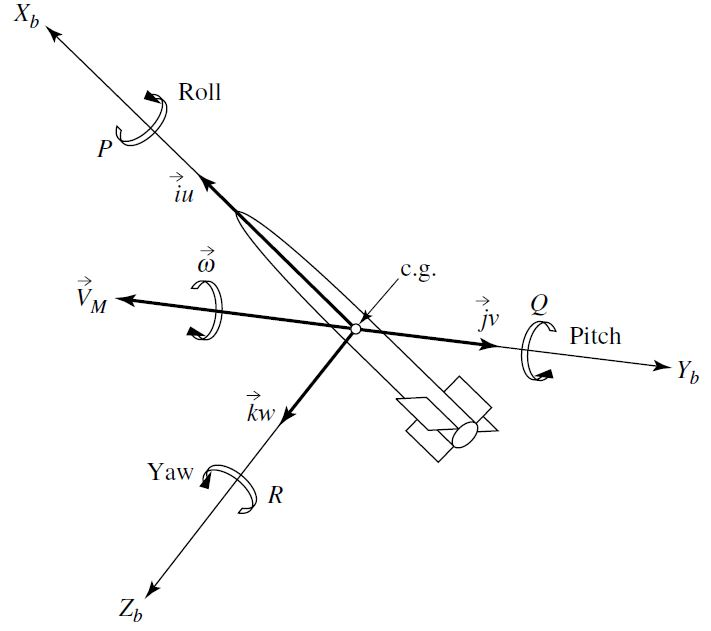
\includegraphics[scale=0.6]{6dof.JPG}
    \caption{Predstava šest stepeni slobode}
    \label{fig:dof}
\end{figure}
Kao što je ranije rečeno dinamički model projektila se dobija Newtonovim zakonom dinamike,
koji kaže da je suma svih vanjskih sila jednaka brzini promjene impulsa tijela i da je 
suma svih vanjskih momenata jednaka brzini promjene moomenta impulsa. Prema tome vrijede relacije:
\begin{equation}
    \sum F=\frac{d(mv_m)}{dt}|_{Zemlja}
    \label{eq:f}
\end{equation}
\begin{equation}
    \sum M=\frac{dH}{dt}|_{Zemlja}
    \label{eq:m}
\end{equation}
gdje je $H$ ugaoni momentum a $\sum M$ je suma svih vanjskih momenata koji djeluju na tijelo. Naravno, prethodne 
relacije predstavljaju promjene vektora u odnosu na inertcijalni prostor. Rezultantna vanjska sila koja 
djeluje na tijelo se može razložiti na sile koje djeluju po osama koordinatnog sistema 
vezanog za tijelo projektila, pa se može napisati:
\begin{equation}
    \sum \Delta F=\sum \Delta  F_xi+\sum \Delta  F_yj+\sum \Delta  F_zk
    \label{eq:sum}
\end{equation}
Poredeći prethodnu jednačinu sa \ref{eq:f} dobija se:
\begin{equation}
    F_x=\frac{d(mu)}{dt}, F_y=\frac{d(mv)}{dt}, F_z=\frac{d(mw)}{dt}
    \label{eq:31}
\end{equation}
Analogno, dobija se da vrijedi:
\begin{equation}
    L=\frac{dH_x}{dt},M=\frac{dH_y}{dt},N=\frac{dH_z}{dt}
    \label{eq:32}
\end{equation}
Gdje su $L,M$ i $N$ moment valjanja, moment propinjanja i moment zakretanja respektivno i 
$H_x, H_y$ i $H_z$ su komponente momenta impulsa duž osa tijela. 
Sada želimo proširiti jednačine \ref{eq:31} i \ref{eq:32} kako bi smo dobili 
jednačine kretanja za svaki stepen slobode. U svrhu toga koristi se formula za 
brzinu promjenu brzine projektila u inercijalnom sistemu, tj. u koordinatnom sistemu 
vezanom za zemlju i ona je data relacijom:
\begin{equation}
    \left( \frac{dv_m}{dt}\right)_{Zemlja}=\left(\frac{dv_m}{dt}\right)_{tijelo}+\omega \times v_m
\end{equation}
Prema tome vrijedi da je ukupna vanjska sila koja djeluje na tijelo data sa:
\begin{equation}
    F=m\left(\frac{dv_m}{dt}\right)_{tijelo}+m(\omega \times v_m)
    \label{eq:force}
\end{equation}
gdje je vektorrski proizvod linearne brzine i ugaone brzine dat sa:
\begin{equation}
    \omega \times v_m=\begin{vmatrix}
        i&j&k\\
        P&Q&R\\
        u&v&w\\
    \end{vmatrix}=(wQ-vR)i+(uR-wP)j+(vP-uQ)k
\end{equation}
Koristeći se činjenicom da je $v_m=ui+vj+wk$ i uvrštavanjem prethodne jednačine u \ref{eq:force} dobija se:
\begin{equation}
    \sum \Delta F=m(\dot{u}i+\dot{v}j+\dot{w}k)+(wQ-vR)i+(uR-wP)j+(vP-uQ)k
\end{equation}
Sada, poredeći sa \ref{eq:sum} dobijaju se jednačine:
\begin{equation}
    \sum \Delta F_x=m(\dot{u}+wQ-vR)
    \label{eq:r1}
\end{equation}
\begin{equation}
    \sum \Delta F_y=m(\dot{v}+uR-wP)
    \label{eq:r2}
\end{equation}
\begin{equation}
    \sum \Delta F_z=m(\dot{w}+vP-uQ)
    \label{eq:r3}
\end{equation}
Prethodno dobivene tri jednačine predstavljaju \textit{linearne jednačine kretanja}. Sada treba odrediti 
ove tri jednačine za rotaciono kretanje. Da bi se to postiglo potrebno je imati izraz za 
moment impulsa $H$ kao što imamo izraz za impuls kod translatornog kretanja. Moment impulsa oko 
proizvoljne tačke $O$ materijalne tačke je dat sa:
\begin{equation}
    H=r\times mV=mr\times (\omega \times r)
\end{equation}
Vektor momenta impulsa $H$ je normalan $r$ i na $v$ i $H$ je usmjeren isto kao i moment impulsa $M$.
Moment impulsa cijelog tijela oko tačke $O$ je dat sa:
\begin{equation}
    H=\sum r\times mv_m=\sum mr\times (\omega \times r)=\sum m\left[\omega(r\cdot r )-r(r\cdot \omega) \right]
\end{equation}
ili u formi integrala:
\begin{equation}
    H=\int r\times (\omega \times r)dm
\end{equation}
Sada slijedi:
\begin{equation}
    \omega \times r=\begin{vmatrix}
        i&j&k\\
        P&Q&R\\
        x&y&z\\
    \end{vmatrix}=(zQ-yR)i+(xR-zP)j+(yP-xQ)k
\end{equation}
 i konačno:
 \begin{equation}
    r\times (\omega \times r)=\begin{vmatrix}
        i&j&k\\
        x&y&z\\
        zQ-yR&xR-zP&yP-xQ\\
    \end{vmatrix}
 \end{equation}
 Sada se konačno dobija izraz za moment impulsa:
 \begin{equation}
    \begin{split}      
     H&=i\int \left[ (y^2+z^2)P -xyQ -xzR \right]dm+j\int\left[ (z^2+x^2)Q-yzR-xyP \right]dm\\ 
     &+k\int \left[ (x^2+y^2)R-xzP-yzQ \right]dm    
    \end{split}
    \end{equation}

    Kada se uvedu oznake:
    \begin{equation}
        \begin{split}           
        I_x&=\int (y^2+z^2)dm, I_z=\int (y^2+x^2)dm,I_z=\int (x^2+z^2)dm\\
        &I_{xy}=\int xydm, I_{yz}=\int yzdm,I_{xz}=\int xzdm 
    \end{split}
    \end{equation}
Tada se dobija:
\begin{equation}
    H=(PI_x-RI_{xz})i+QI_yj+(RI_z-PI_{xz})k
\end{equation}
Sada se vektor momenta impulsa može zapisati preko svojih komponenti:
\begin{equation}
    H_x=PI_x-RI_{xz}
\end{equation}
\begin{equation}
    H_y=QI_y
\end{equation}
\begin{equation}
    H_z=RI_z-PI_{xz}
\end{equation}
Sada su potrebni izvodi momenta impulsa kako bi smo dobili izraz za rezultantni moment.
Pošto je izvod vektora u inercijalnom prostoru jednak zbiru izvoda pojedinačnih komponenti vektora. Prema tome 
vrijedi:
\begin{equation}
    \frac{dH_x}{dt}=I_x\frac{dP}{dt}-I{xz}\frac{dR}{dt}
\end{equation}
\begin{equation}
    \frac{dH_y}{dt}=I_y\frac{dQ}{dt}
\end{equation}
\begin{equation}
    \frac{dH_z}{dt}=I_z\frac{dR}{dt}-I_{xz}\frac{dP}{dt}
\end{equation}
Relacija \ref{eq:m} se može napisati kao:
\begin{equation}
    \sum \Delta M=\frac{dH}{dt}+\omega \times H
\end{equation}
Ako se uvaži da je $\sum \Delta M=\sum \Delta Li + \sum \Delta Mj+\sum \Delta Nk$, korištenjem prethodno dobivenih 
izraza za izvod momenta impulsa dobija se:
\begin{equation}
    \sum \Delta L=\dot{P}I_x+QR(I_z-I_y)-(\dot{R}+PQ)I_{xz}
\end{equation}
\begin{equation}
    \sum \Delta M=\dot{Q}I_y+PR(I_x-I_z)+(P^2-R^2)I_{xz}
\end{equation}
\begin{equation}
    \sum \Delta N=\dot{R}I_y+PQ(I_y-I_x)-(\dot{P}-QR)I_{xz}
\end{equation}
Prethodne tri jednačine zajedno sa jednačinama \ref{eq:r1},\ref{eq:r2} i \ref{eq:r3} predstavljaju
jednačine projektila sa šest stepeni slobode. Ove jednačine su simultane linearne jednačine 
kretanja sa šest promjenjivih $u,v,w,P,Q$ i $R$ koje potpuno opsiuju kretanje 
čvrstog tijela. Rješenja ovih jednačina se mogu dobiti numeričkim metodama na digitalnom 
računaru. Analitička rješenja dovoljne tačnosti se mogu dobiti linearizacijom. $I_x,I_y$ i $I_{xz}$ su konstantne 
i za projektile sa krstastom konfiguracijom vrijedi $I_y=I_z$ i $I_{xz}$. Prema tome, vrijedi:
\begin{equation}
    \sum \Delta L=\dot{P}I_x+QR(I_z-I_y)
\end{equation}
\begin{equation}
    \sum \Delta M=\dot{Q}I_y+PR(I_x-I_z)
\end{equation}
\begin{equation}
    \sum \Delta N=\dot{R}I_z+PQ(I_y-I_x)
\end{equation}
Transformacijom prethodnih jednačina dobija se:
\begin{equation}
    \frac{dP}{dt}=QR\frac{I_y-I_z}{I_x}+\frac{L}{I_x}
    \label{eq:q1}
\end{equation}
\begin{equation}
    \frac{dQ}{dt}=PR\frac{I_z-I_x}{I_y}+\frac{M}{I_y}
    \label{eq:q2}
\end{equation}
\begin{equation}
    \frac{dR}{dt}=PQ\frac{I_x-I_y}{I_z}+\frac{N}{I_z}
    \label{eq:q3}
\end{equation}
Sada je još potrebno odrediti ugaone brzine u zavisnosti od Eulerovih uglova. Izvođenje ovih jednačina zahtjeva 
pronalaženje izvoda matrice transformacije, što je poprilično zahtjevno, pa će ovdje biit samo navedene 
diferencijalne jednačine koje daju brzinu prmjene Eulerovih uglova:
\begin{equation}
    \frac{d\psi}{dt}=(Q\sin\phi +R\cos\phi)/\cos\theta
    \label{eq:w1}
\end{equation}
\begin{equation}
    \frac{d\theta}{dt}=Q\cos\phi-R\sin\phi
    \label{eq:w2}
\end{equation}
\begin{equation}
    \frac{d\phi}{dt}=P+\left( \frac{d\psi}{dt} \right)\sin\theta
    \label{eq:w3}
\end{equation}
Sada koristeći matricu transformacije $C_e^b$ se mogu dobiti komponente
brzine u koordinatnom sistemu Zemlje:
\begin{equation}
    \begin{bmatrix}
        \dot{X_z}\\
        \dot{Y_z}\\   
        \dot{Z_z}\\
    \end{bmatrix}=C_e^b\begin{bmatrix}
        u\\
        v\\   
        w\\
    \end{bmatrix}
    \label{eq:q}
\end{equation}
Sada je jasno da se integracijom jednačina \ref{eq:q1},\ref{eq:q2} i \ref{eq:q3} dobijaju 
ugaone brzine u sistemu tijela, a integracijom jednačina \ref{eq:w1},\ref{eq:w2} i \ref{eq:w3}  se dobija 
orijentacija u odnosu na zemlju. Da bi se dobila pozicija tijela u odnosu na sistem Zemlje
treba riješiti matričnu jednačinu \ref{eq:q}. Da bi se ona mogla numerički riješiti treba 
naći izraze za izvode brzinu u sistemu tijela. Oni se mogu dobiti iz jednačina 
\ref{eq:r1}, \ref{eq:r2} i \ref{eq:r3}. Nakon transformacije ovih jednačina ima se:
\begin{equation}
    \frac{du}{dt}=vR-wQ+F_x/m
\end{equation}
\begin{equation}
    \frac{dv}{dt}=wP-uR+F_y/m
\end{equation}
\begin{equation}
    \frac{dw}{dt}=uQ-vR+F_z/m
\end{equation}
Sada se nakon rješavanja prethodne tri jendačine mogu dobiti vrijednosti brzina u sistemu tijela 
te nakon toga može se riješiti jednačina \ref{eq:q} i tako dobiti poziciju u odnosu na sistem Zemlje.
Prethodnih 12 jednačina se može predstaviti u prostoru stanja ako se uzme vekor varijabli stanja:
\[\vec{X}=\left[ u \quad v\quad w\quad P\quad Q\quad R\quad \phi \quad \theta \quad
 \psi \quad x_z\quad y_z\quad z_z\quad \right]^T\] i vektor upralvjačkih 
promjenljivih:
\[\vec{u}=\left[\delta_v \quad \delta_P\quad \delta_e \right]^T\] 
,gdje je $\delta_v$ ugao otklona krmila visine, $\delta_P$, ugao otklona krmila 
i $\delta_e$, ugao toklona elerona. Upravljačke varijable se na prvu ruku ne vide i predstalvjenim jednačinama, 
ali ubrzo ćemo se uvjeriti da sile i momenti koji djeuluju na projektil zavise upravo od ovih upralvjačkih 
varijabli.  
Ovime se dobija nelinearna vekotrska jednačina:
\begin{equation}
    \dot{\vec{X}}=f(\vec{X},\vec{u},t)
\end{equation}
Prethodna jednačina je doista nelinearna najprije zbog prirode modela, postojanja trigonometrijskih funkcija i 
zbog nelinearne zavisnosti sila i momenata od otklona upralvjačkih površina. Kako bi se izvršila sinteza 
regulatora prethodna jednačina se najprije treba linearizirati za određeni režim leta. Već se nadzire 
da se linearizacija može izvršiti nalaženjem prvih izvoda vekotrske funkcije $f(\vec{X},\vec{u},t)$ za određene uslove leta. 
Dobijena matrica bi imala 144 elementa koji su u stvari prvi izvodi raznih parametara modela pa je evidentno 
da treba poznavati zavisnosti parametra od vremena i međusobne zavisnosti varijabli stanja.  







\chapter{Sile koje djeluju na projektil}

Sile koje djeluju na projektil su u letu su aerodinamičke, pogonske sile i 
gravitaciona sila. Ove sile se mogu razložiti po osama kooridnatnog sistema vezanog 
za tijelo. 
\section{Aerodinamičke sile}
Aerodinamička sila je posljedica djelovanja pritiska okolnog fluida na tijelo u pokretu. 
Aerodinamička sila se može razložiti na tri komponente koje su definisane u nastavku:
\begin{itemize}
    \item \textbf{Uzgon}- Uzgon je komponenta rezultantne aerodinamičke sile 
    koja je normalna na relativno kretanje vjetra.
    \item \textbf{Otpor}- Otpor je komponenta rezultantne aerodinamičke sile 
    koja je paralelna relativnom kretanju vjetra.
    \item \textbf{Bočna sila}- Bočna sila je komponenta rezultantne aerodinamičke sile 
    koja je normalna na uzogn i otpor. 
\end{itemize}
Ovdje se posmatraju projektili koji se zakreću da bi skrenuli(skid to turn) i 
kod takvih projektila aerodinamičke sile su date sa:
\begin{equation}
   \text{Otpor} \quad R_x=C_xqS
   \label{eq:aa1}
\end{equation}
\begin{equation}
    \text{Uzgon} \quad R_z=C_zqS
    \label{eq:aa2}
\end{equation}
\begin{equation}
    \text{Bočna sila} \quad R_y=C_yqS
    \label{eq:aa3}
\end{equation}
,gdje su $C_x,C_y$ i $C_z$ aerodinamički koeficijenti, $q$ dinamički pritisak slobodnog strujanaja
u tački daleko od objekta i iznosi $q=\frac{1}{2}\rho v^2$, $S$ je referentna površina i 
$v$ je brzina vazduha, $\rho$ predstavlja atmosferski pritisak.
\\
Treba napomenuti da se aerodinamičke sile i momenti izražavaju bezdimenzionalnim veličinama. 
To se postiže tako što se dogovorom utvrdi da se sila(ili moment) predstavlja svojim odgovarajućim 
aerodinamičkim koeficijentom. Prema tome, $C_x$ potpuno određuje silu otpora i slično vrijedi i 
za ostale koeficijente. \\

U opštem slučaju koeficijenti aerodinamičkih sila su funkcije varijabli stanja pa se može
napisati:
\begin{equation}
    C_x=C_x(\alpha ,\beta, M,q,\delta_v,\delta_P,\delta_e)
\end{equation}
,gdje je $M$ Mahov broj- odnos tekuće brzine i brzine zvuka, $\alpha$ napadni ugao i 
$\beta$ ugao klizanja. Slično tako vrijedi:
\begin{equation}
    C_z=C_z(\alpha ,\beta, M,q,\delta_v,\delta_P,\delta_e)
\end{equation}
Uglovi $\alpha, \beta$ i $\gamma$ su prikazani na slici \ref{fig:angles} i definisani su sa:
\begin{equation}
    \alpha=arctg(w/u)
\end{equation}
\begin{equation}
    \beta=\arcsin(v/v_m)
\end{equation}
\begin{figure}[ht!]
    \centering
    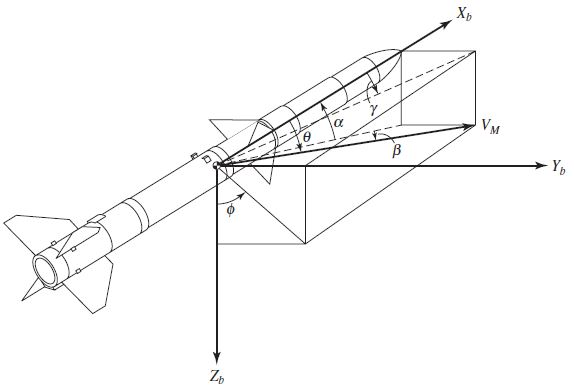
\includegraphics[scale=0.7]{angles.JPG}
    \caption{Ugaone veze}
    \label{fig:angles}
\end{figure}
Razvojem u Taylorov red i odbacivanjem viših članova dobija se aproksimacija 
aerodinamičkih koeficijenata:
\begin{equation}
    C_x=C_{x_0}+C_{x_\alpha}|\alpha|+C_{x_\alpha^2}\alpha^2+C_{x_\beta}|\beta|+
    C_{x_\beta^2}\beta^2+C_{x_\alpha \beta}|\alpha||\beta|
\end{equation}
\begin{equation}
   C_z=C_{z_0}+C_z^{\alpha}{\alpha} + C_z^{\dot{\alpha}} \dot{\alpha}+C_z^q q+C_z^{\delta _v}{\delta _v}
\end{equation}
\begin{equation}
    C_y=C_{y_0}+C_y^{\alpha}{\alpha} + C_y^{\dot{\alpha}} \dot{\alpha}+C_y^q q+C_y^{\delta _v}{\delta _v}
\end{equation}
U datom slučaju aerodinamički koeficijent otpora imaju jednostavniji oblik
\begin{equation}
    C_x=C_{x_0} + C_{x_1}\alpha
\end{equation}
,gdje je $C_{x_0}=\frac{\partial c_x}{\partial \alpha}|_{\alpha=0}$, $C_{x_1}=\frac{\partial c_x}{\partial \alpha}$ 
i slično tako za ostale izvode.\\
Također je važno istaći da su ovi koeficijenti(tj. sile) izražene u \textit{kooridnatnom sistemu vjetra} 
relativnom toku vazduha. Koordinatni sistem vazduha je prikazan na slici \ref{fig:wind}. 
\begin{figure}[ht!]
    \centering
    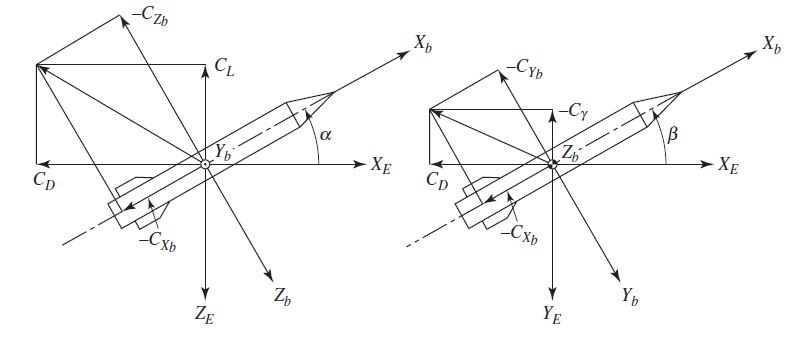
\includegraphics[scale=0.5]{wind.JPG}
    \caption{Veza između sistema tijela i sistema vjetra}
    \label{fig:wind}
\end{figure}
Pošto su jednačinama kretanja tijela sile izražene sistemu tijela, potrebno
je imati transformaciju koja transformiše aerodinamičke sile u sistem tijela i njihova veza je data sa:
\begin{equation}
    \begin{bmatrix}
        C_{x_b}\\
        C_{y_b}\\
        C_{z_b}\\
    \end{bmatrix}=\begin{bmatrix}
        \cos\alpha && -\cos\alpha && \sin\alpha\\
        \sin\beta &&\cos\beta && 0\\
        \sin\alpha\cos\beta && -\sin\alpha\sin\beta && \cos\alpha\\
    \end{bmatrix}\begin{bmatrix}
        -C_x\\
        C_y\\
        -C_z\\
    \end{bmatrix}
\end{equation} Sada se vraćanjem u \ref{eq:aa1},\ref{eq:aa2} i \ref{eq:aa3} mogu odrediti 
aerodinamičke sile koje djeluju na projektil. 
\section{Aerodinamički momenti}
Momenti se mogu podjeliti na momente koji su posljedica aerodinamičkog tereta i 
pogonske sile koja ne djeulje kroz centar gravitacije. Moment koji je posljedica 
rezultantne sile koja ne djeluje na centar kooridnatnog sistema tijela se može 
podjeliti na tri komponente, i to:
\begin{itemize}
    \item \textbf{Moment valjanja} je moment oko lateralne ose($Y_b$) projektila i generisan 
    je od uzgonom i otporom koje djeluju na tijelo. Pozitivan moment je u smjero gore 
    od nosa letjelice 
    
    \item \textbf{Moment propinjanja} je moment oko longitudinalne ose($X_b$) projektila.
    Posljedica je uzogna koji je uzrokovan nekom vrstom elerona. Pozitivan moment propinjanja uzrokuje kretanje nadole 
    desnog krila.
    
    \item \textbf{Moment zakretanja} je moment oko vetikalne ose projektila($Z_b$). Pozitivan moment zakretanja 
    ima za posljedicu da se nos aviona zakrene u desno. 
\end{itemize}
Kvantitativno, momenti su dati sa:
\begin{equation}
    \text{Moment valjanja} \quad L=C_lqSb
    \label{eq:a1}
 \end{equation}
 \begin{equation}
     \text{Moment propinjanja} \quad M=C_mqSc
     \label{eq:a2}
 \end{equation}
 \begin{equation}
     \text{Moment zakretanja} \quad N=C_nqSb
     \label{eq:a3}
 \end{equation}
 ,gdje je $b$ raspon krila, $c$ je razmak između početne i krajnje ivice krila mjerene 
 u smjeru paralelnom toku vazduha, $S$ je površina platforme krila. 
 Isto kao i kod slučaja sa silama, koeficijenti momenata također zavise od više promjenjivljih 
 i potrebno ih je linearizirati. \\
 Linearizirani koeficijenti momenta su:
 \begin{equation}
     C_m=C_m^{\alpha}\alpha +C_m^{\dot{\alpha}}\dot{\alpha } + C_m^q q+C_m^{\delta _v}\delta _v
 \end{equation} 
 ,i koeficijent momenta valjanja:
 \begin{equation}
     C_L = C_l^PP+C_l^QQ+C_l^RR +C_l^\alpha \alpha +C_l^\beta \beta + C_l^{\delta _e} \delta _e +C_l^{\delta _v} \delta _v
     +C_l^{\delta _P} \delta _P
 \end{equation}

\chapter{Dinamički model}
Potpun nelinearni dinamički model sastoji iz 12 diferencijalnih jednačina koje su predstavljene ranije. 
Iznimno je teško dobiti analitičko rješenje ovih diferencijalnih jednačina pa se obično pribjegava numeričkoj
simulaciji modela. Zadatak autopilota je da osigura brz prelaz stanja i stabilan odziv u okolini nominalne trajektorije. 
Pokazaće se da se za nominalnu trajektoriju čitav model može raspregnuti što ima za posljedicu 
potpuno razdvajanje modela na dva podsistema. Ova praksa je korištena kod starih letjelica zbog 
uštede računarske moći, ali to danas više nije problem zbog razvoja digitalnih račuara, međutim rasprezanje 
dinamičkog modela je i danas korisno u svrhu sinteze regulatora. Rasprezanje dinamičkog modela 
uvodi netačnosti u model pošto je za rasprezanje potrebno zanemarivanje određenih veličina pa se 
preporučuje ispitivanje regulatora na nelinearnom modelu. U nastavku su sumarno prikazane ranije izvedene 
relacije koje opisuju model projektila krstaste konfiguracije pri čemu treba primjetiti da su ove jednačine 
sada prikazane u koordinatnom sistemu brzine. Korišten je indeks $v$(velocity) da se označi vektor u sistemu brzine
i indeks $b$(body) da se označi vekor u sistemu tijela. Da bi se transformisao vektor iz sistema tijela u sistem brzine 
treba se koristiti inverz matrice transformacije date sa \ref{eq:VtoB}, koji iznosi:
\begin{equation}
    T_b^v = \begin{bmatrix}
            \cos\beta & \sin\beta & 0\\
            -\sin\beta & \cos\beta & 0\\
            0 & 0& 1\\
        \end{bmatrix}
        \begin{bmatrix}
            \cos\alpha & 0 & -\sin\alpha \\
        0& 1& 0\\
        \sin\alpha & 0 & \cos\alpha
        \end{bmatrix}
\end{equation}
Nakon množenja matrica dobija se:
\begin{equation}
    T_b^v\begin{bmatrix}
        \cos\alpha\cos\beta & \sin\beta & -\sin\alpha\cos\beta \\
        -\cos\alpha\sin\beta & \cos\beta & \sin\alpha\sin\beta \\
        \sin\alpha & 0 & \cos\alpha
    \end{bmatrix}
\end{equation}
Sada se konačno može napisati svih 12 diferencijalnih jednačina modela u koordinatnom sistemu brzine.
\begin{align}
    &\frac{dV}{dt} = \frac{F_{xv}}{m}\\
    &\frac{d\Psi}{dt} = \frac{F_{yv}}{mV\cos\Theta}\\
    &\frac{d\Theta}{dt} = -\frac{F_{zv}}{mV}\\
    &\frac{dP}{dt}=L/I_x\\
    &\frac{dQ}{dt}=[M+(I_z-I_x)RP]/I_y\\
    &\frac{dR}{dt}=[N+(I_x-I_y)PQ]/I_z\\
    &\frac{d\psi}{dt}=(R\cos\phi+Q\sin\phi)/\cos\theta\\
    &\frac{d\theta}{dt}=Q\cos\phi-R\sin\phi\\
    &\frac{d\phi}{dt}=P+(R\cos\phi+Q\sin\phi)\tan\theta\\
    &\frac{dx_z}{dt}=V\cos\Theta\cos\Psi\\
    &\frac{dy_z}{dt}=V\cos\Theta\sin\Psi\\
    &\frac{dz_z}{dt}=V\sin\Theta
\end{align}
Ovaj nelinearni model ima tri ulaza(otkloni kontrolnih površina) i svaka od varijabli stana može izlaz pa se kod lineariziranog 
modela može predstaviti 36 prenosnih funkcija, međutim zbog prirode posmatrane konfiguracije 
neke od ovih prenosnih funkcija će identički biti jednake nuli. Jedan primjer ovakve prensone funkcije 
jeste veza između otklona upravljačke površine za stabilizaciju ugla valjanja i brzine projektila. 
U prethodnom poglavlju su razvijeni izrazi za sile u koordinatnom sistemu tijela, pa su u nastavku navedene 
jednačine koje opisuju model u koordinatnog sistemu tijela:
\begin{align}
    \label{eq:prva} \frac{du}{dt} &=Rv - Qw + (F_{ax} + F_{gx} + T)/m\\
    \frac{dv}{dt} &=Pw - Ru + (F_{ay}+F_{gy})/m\\
    \frac{dw}{dt} &=Qu - Pv +(F_{az}+F_{gz})/m\\
    \frac{dP}{dt} &=L/I_x\\
    \frac{dQ}{dt} &= PR\frac{I_z-Ix}{Iy} + M/I_y\\
    \frac{dR}{dt} &= PQ\frac{I_x-IY}{Iy} + N/I_z\\
    \frac{d\phi}{dt} &=P + Q\sin\phi\tan\theta + R\cos\phi\tan\theta\\
    \frac{d\theta}{dt} &=Q\cos\theta - R\sin\phi\\
    \label{eq:zadnja} \frac{d\psi}{dt}&=(R\cos\phi+Q\sin\phi)/\cos\theta
\end{align}
Ovakav prikaza dinamičkog modela je naročito koristan za simulaciju dinamike projektila. 
\section{Softverska implementacija modela}
Od velike je koristi imati implementiran dinamički model kako bi se imao bolji 
uvid u dinamiku projektila. Također neophodno je imati implementiran 
nelinearni model za potrebe dizajna linearnih regulatora. Regulatori su linearni, ali 
je potrebno imati i uvjerljiv nelinarni model kako bi se ispitale performanse regulatora.
Dinamički model je implementiram koristeći Matlab i Simulink polazeći od jednostavne ideje,
da se koristeći prethodno dobivene izraze, izračunaju izvodi varijabli stanja te da se one 
nakon toga integrale čime se dobijaju stvarne vrijednosti varijabli stanja. Riješene su jednačine 
od \ref{eq:prva} do \ref{eq:zadnja} uz izraze za ugao napada i ugao klizanja. 
Prisjetimo se da vrijedi:
\begin{align*}
    \alpha &= \arctan(\frac{w}{v})\\
    \beta &= \arctan(\frac{v}{u})
\end{align*}
Prema tome, vrijedi:
\begin{align}
    \dot{\alpha} &= \frac{u\dot{w} - w\dot{u}}{w^2+v^2}\\
    \dot{\beta} &= \frac{u\dot{v} - v\dot{u}}{u^2+v^2}
\end{align}
Također je korištena činjenica da vrijedi:
\begin{align}
    \Theta &= \theta - \alpha\\
     \Psi &= \psi - \beta
\end{align}
Iz čega se mogu dobiti vertikalno i horizontalno ubrzanje vezano za koordinatni sistem prema relacijama:
\begin{align}
    a_V &= v_m\dot{\Theta} + g\cos\Theta \\
    a_H &= v_m\dot{\Psi}\cos\Theta 
\end{align}
Ova dva ubrzanje su normalna na vektor brzine projektila. \\
U nastavku je prikazan simulink dijagram koji služi kao nelinarni model projektila sa 
šest stepeni slobode. 
\begin{figure}[!ht]
    \centering
    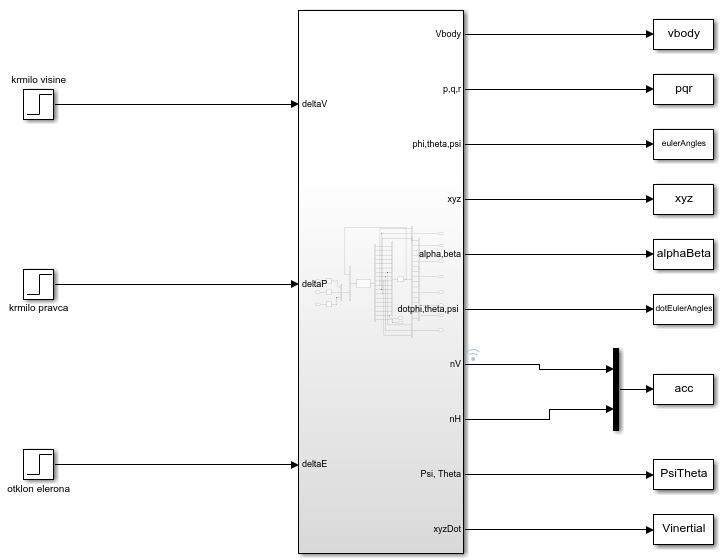
\includegraphics[scale=0.7]{model.JPG}
    \caption{Simulink model projektila}
\end{figure}
Na prethodnoj slici je predstavljen podsistem koji iza sebe krije pravu dinamiku projektila. 
Na narednoj slici je prikazan ovaj podsistem. 
\begin{figure}[!ht]
    \centering
    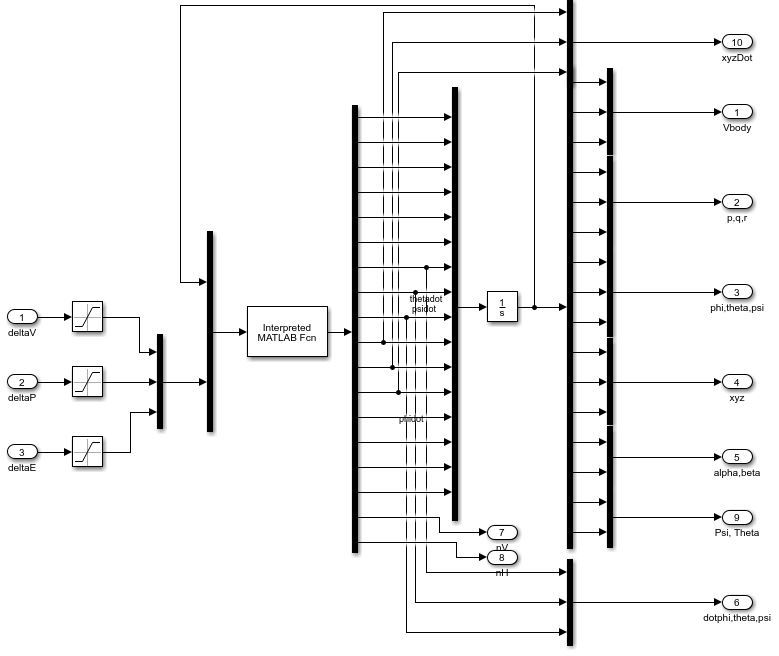
\includegraphics[scale=0.7]{subModel.JPG}
    \caption{Simulink model projektila}
    \label{fig:subimg}
\end{figure}
Na slici \ref{fig:subimg} se vidi da je kod modela u obzir uzeto da se može postići samo 
konačan otklon kontrolnih površina. Dalje, koristi se blok interpretirane Matlab funkcije 
kako bi se riješile simultane diferencijalne jednačine modela, koje se prosljeđuju 
u integrator sa određenim početnim uslovima. Također ova interpretirana funkcija računa 
i normalno i vertikalno ubrzanje projektila, kao i ugao elevacije i azimuta vektora brzine. Dakle,
ova interpretirana Matlab funkcija kao ulaze ima sve varijable stanja, napadni ugao $\alpha$ i ugao klizanja $\beta$, 
ugao elevacije vektora brzine $\Theta$, ugao azimuta vektora brzine $\Psi$ i otklone 
upravljačkih površina. U nastavku je prikazan Matlab kod interpretirane funckije koja 
rješava jednačine dinamičkog modela. 
\begin{lstlisting}
    function out = modelSolver(X,alpha,beta,Psi, Theta, U)
    
    u = X(1);
    v = X(2);
    w = X(3);
    p = X(4);
    q = X(5);
    r = X(6);
    phi = X(7);
    theta = X(8);
    psi = X(9);
    
    xz = X(10);
    yz = X(11);
    zz = X(12);
    
    u1 = U(1);
    u2 = U(2);
    u3 = U(3);
    
    %------------CONSTANTS-------------------%
    m = 52.5;
    Ix = 0.16;
    Iy = 14;
    Iz = Iy;
    g= 9.81;
    l = 0.127;
    rho = 1.225;
    D = 127/1000;
    S = 0.0127;
    vm = sqrt(u^2+v^2+w^2);
    
    Q = (rho*(vm^2))/2;
    %----------COEFFICIENTS--------------------%
    
    %lift
    
    Cx0 = 10;
    Cna = 3.330;
    
    Fa = -rho*pi*D^2*vm^2*[Cx0+alpha^2 + beta^2;Cna*beta;Cna*alpha]/8;
    
    Fax = Fa(1);
    Fay = Fa(2);
    Faz = Fa(3);
    %moments
    
    X = 0.55;
    
    Cma = -Cna*X/l;
    CmdeltaV = 10;
    
    Cmq = -300;
    Cm = Cma*alpha + CmdeltaV*u1 + Cmq*q/(2*vm);
    
    Mm = Cm*Q*S*l;
    
    Cnb = -Cma;
    CndeltaP = -CmdeltaV;
    Cnr = -300;
    Cn = Cnb*beta + CndeltaP*u2 + Cnr*r/(2*vm);
    Nm = Cn*Q*S*l;
    
    
    CldeltaE = 1.4;
    Clp = -9;
    
    Cl = CldeltaE*u3 + Clp*p/(2*vm);
    Lm = Cl*Q*S*l;
    
    Tphi = [1 0 0;
            0 cos(phi) sin(phi);
            0 -sin(phi) cos(phi)];
    Ttheta = [cos(theta) 0 -sin(theta);
              0 1 0;
              sin(theta) 0 cos(theta)];
    Tpsi = [cos(psi) sin(psi) 0;
            -sin(psi) cos(psi) 0;
            0 0 1];
    
    Thrust = 12650;
    udot = v*r - w*q + (Fax+Thrust)/m -g*sin(theta);
    vdot = p*w - r*u + Fay/m + g*cos(theta)*sin(phi);
    wdot = q*u - p*v + Faz/m + g*cos(theta)*cos(phi);
    
    pdot = Lm/Ix;%pdot
    qdot = p*r*(Iz-Ix)/Iy +Mm/Iy;%qdot
    rdot = p*q*(Ix-Iy)/Iz + Nm/Iz;%rdot
    
    phidot = p+q*sin(phi)*tan(theta)+r*cos(phi)*tan(theta);
    thetadot = q*cos(phi) - r*sin(phi);
    psidot = q*sin(phi)/cos(theta) + r*cos(phi)/cos(theta);
    
    xyzZemlja = Tpsi'*Ttheta'*Tphi'*[u;v;w];
    
    Xdot = [udot;vdot;wdot;pdot;qdot;rdot;phidot;thetadot;psidot;xyzZemlja];
    
    alphadot = (wdot*u - udot*w)/(w^2+u^2);
    betadot = (vdot*u - v*udot)/(u^2+v^2);
    
    Thetadot = thetadot-alphadot;
    Psidot = psidot - betadot;
    
    nV = vm*Thetadot + g*cos(Theta);
    nH = vm*Psidot*cos(Theta);
    
    out = [Xdot; alphadot; betadot;Psidot;Thetadot;nV;nH];
    end
    \end{lstlisting}
Model projektila je MIMO sistem sa tri ulazne varijable i puno više izlaze pa je u nastavku 
predstavljeno nekoliko značajnih odziva na otklone kotnrolnih površina. U nastavku se razmatra 
šta se dešava sa projektilom kada se pobudi sa jediničnim otklnom krmila visine. Treba uzeti u obzir 
da je uzeto u modelu da se postiže zasićenje otklona svih površina pri otklonu od $25$ stepeni.
Prvo pogledajmo šta se desi sa orijentacijom projektila za jedinični otklon krmila visine. 
\begin{figure}[!ht]
    \centering
    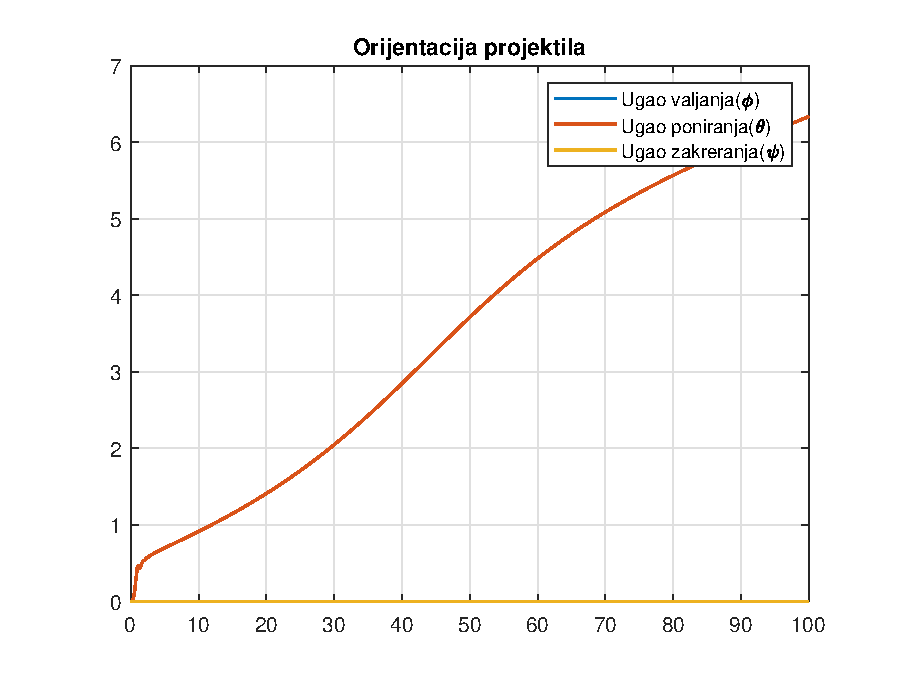
\includegraphics[scale = 0.5]{pitchVis.eps}
    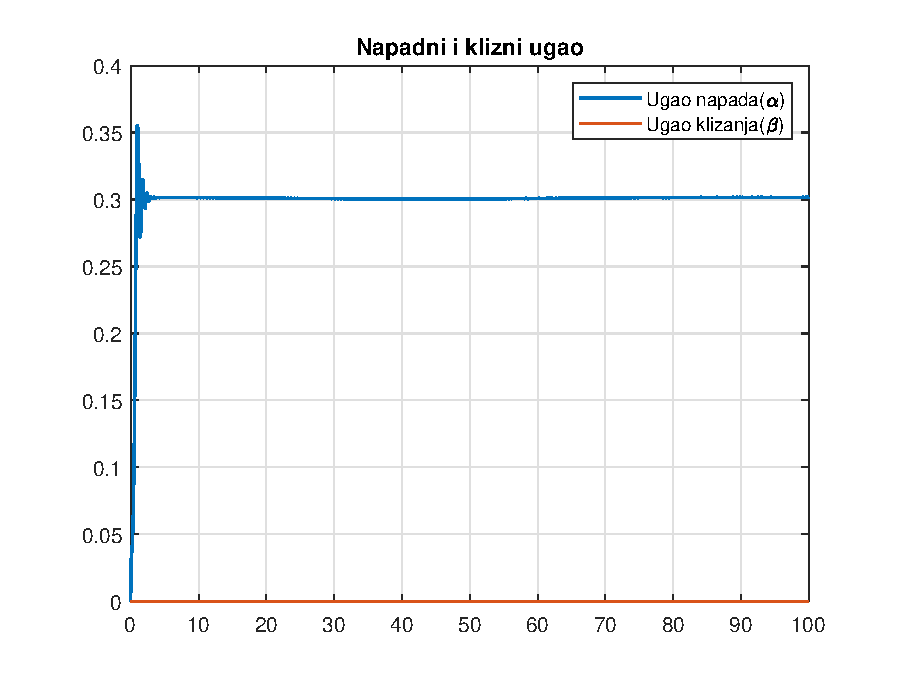
\includegraphics[scale = 0.5]{AoAvis.eps}
    \caption{Orijentacija projektila i ugao napada i klizanja pri jediničnom otklonu krmila 
    visine}
\end{figure}
Sada se vide očekivani rezultati. Kada se otkloni krmilo visine, projektil se usmjeri lagano prema gore. 
Grafik na kojem je prikazan ugao propinjnanja je dat u radijanima, pa se prema skoro linearnom 
odzivu može naslutiti da je putanja projektila kružne prirode. U ovu tvrdnju ćemo se uvjeriti poslije. Dalje,
vidimo da je napadni ugao konstantan u toku cijele putanje, što znači da se projektil uvijek kreće u smjeru $z$ ose tijela.
Ovo ne znači nužno da se projektil penje. Dalje, ugao klizanja je nula toko cijele putanje što 
znači da projektil ne skreće sa putanje, tj. da je vrijednost pomjeraja po $y$ osi uvijek nula. To se također 
vidi na graficima za ugao zakretanja. Treba primjetiti da je ugao valjanja također nula za jedinični otklon 
krmila visine. Ovo su itekako važni zaključci, jer se primjećuje da otklon krmila visine uzrokuje 
kretanje samo u vertikalnoj ravni pa se već naslućuje da postoji nezavisnost kretanja u vertikalnoj i horiznotalnoj 
ravni. Poslije ćemo se uvjeriti da je ova osobina od krucijalne važnosti za dizajn autopilota za zadatak vođenja. 
Sada pogledajmo, odzive brzina projektila koji su prikazani na slici \ref{fig:brzine}.
\begin{figure}[!ht]
    \centering 
    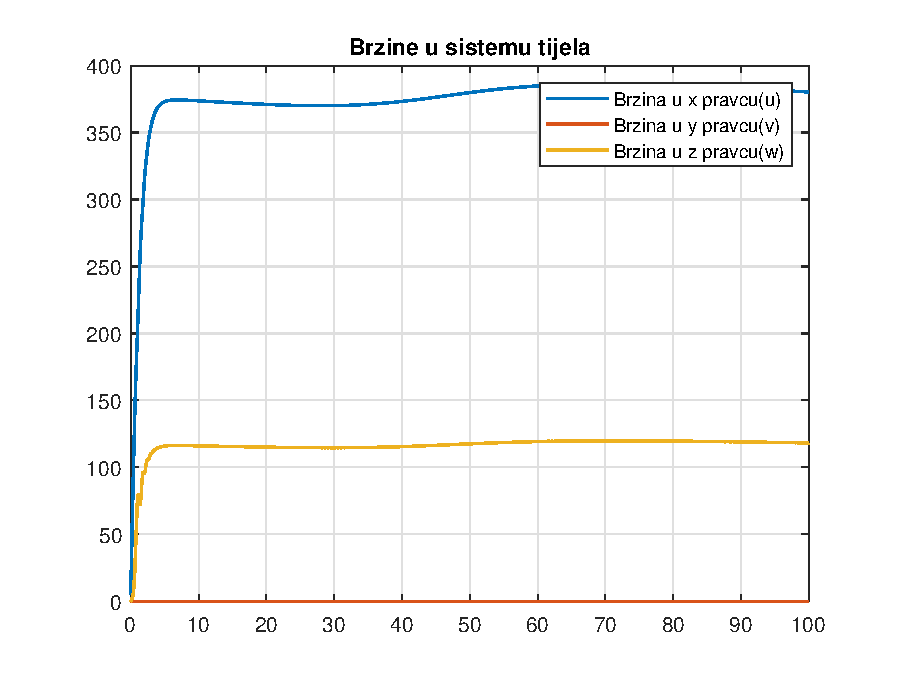
\includegraphics[scale =.5]{VbodyVis.eps}
    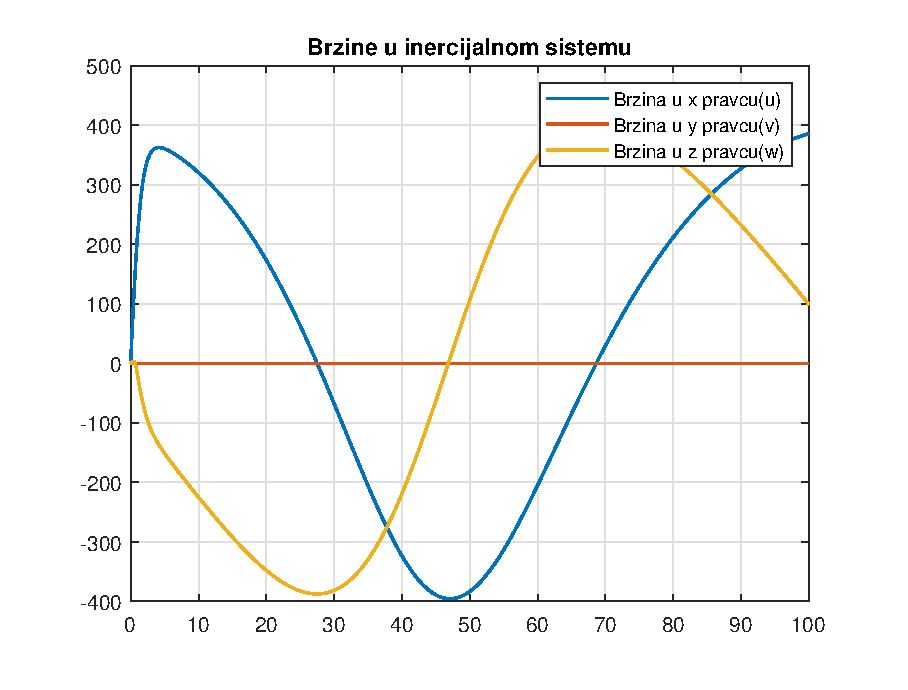
\includegraphics[scale =.5]{VinVis.eps}
    \caption{Brzine projektila u sistemu tijea i inercijalnom sistemu}
    \label{fig:brzine}
\end{figure}
Prvo što se primjeti jest da je brzina u $y$ smjerovima oba sistema uvijek nula. Dalje, posmatrajući 
sistem tijela vidi se da brzine nakon nekog vremena dostignu maksimalnu brzinu. Glede,
sistema tijela, brzina u $x$ smjeru je stalna kao posljedica čeone sile otpora vazduha. Posmatrajući
inercijalni sistem, vidi se brzine u $x$ i $z$ smjeru imaju promejene koje sliče na kružno kretanje. Suma njihovih kvadrata 
će dati približno neku konstantnu vrijednost, pa se zaključuje da se projektil za slulčaj otklona krmila visine, 
doista kreće po kružnici. Uvjerimo se u tu tvrdnju skicirajući putnaju projektila. Čitalac treba 
da primjeti da je na ovoj slici izvršena promjena znaka visine projektila. 
\begin{figure}[!ht]
    \centering 
    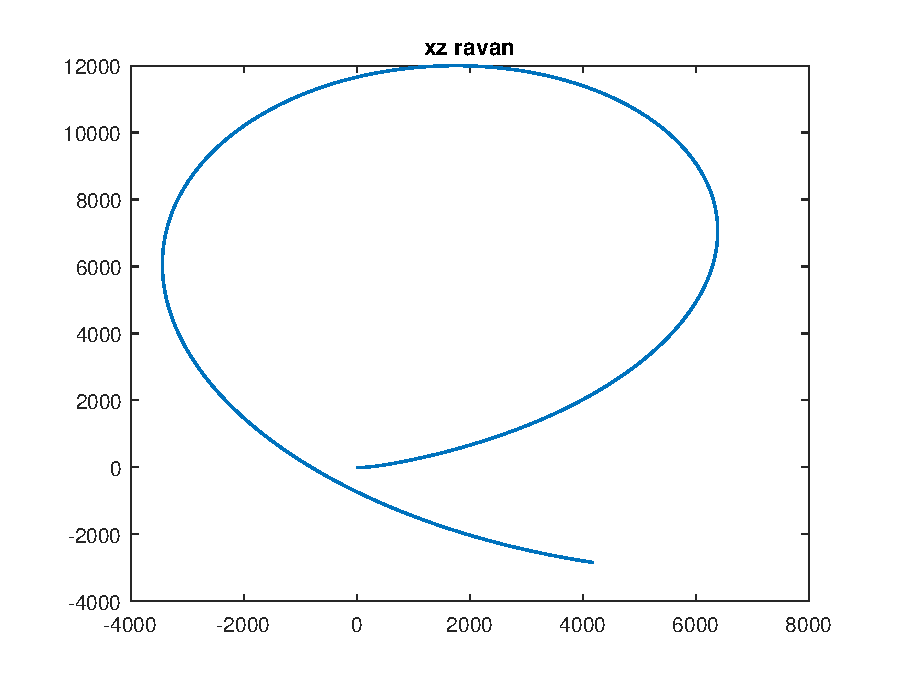
\includegraphics[scale= 0.5]{putnja2Dvis.eps}
    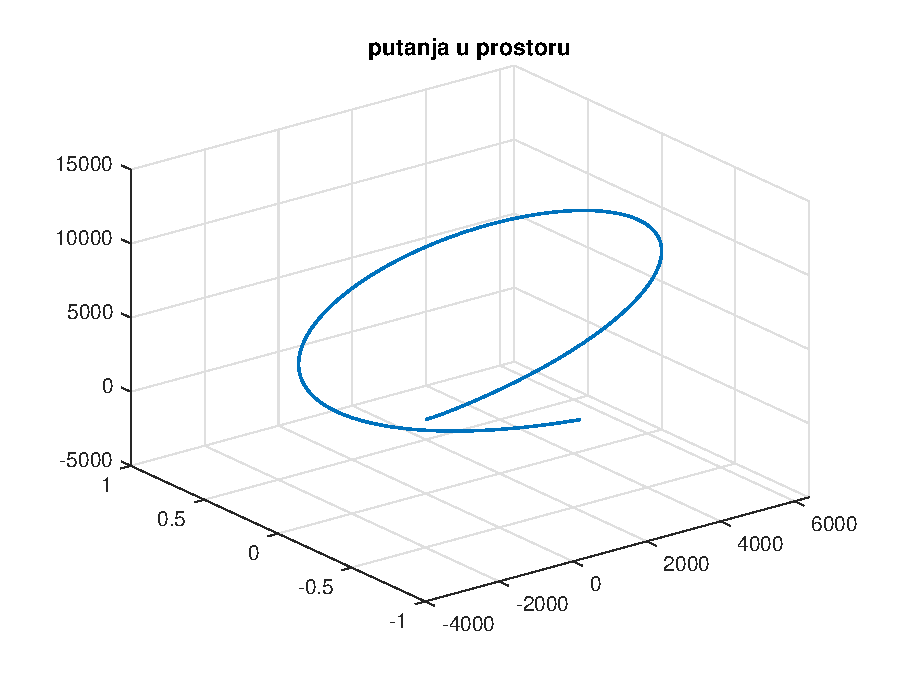
\includegraphics[scale= 0.5]{3dputanjaVis.eps}
    \caption{Putanja projektila za jedinični otklon krmila visine}
    \label{fig:2dpath}
\end{figure}
Sada se jasno vidi da projektil pravi kružnu putanju u prostoru. 
Poslije će se vidjeti da su normalna ubrzanje važna za proces vođenja projektila, pa treba razmotriti 
šta se dešava sa ubrzanjima kada se imaju otkloni kontrolnih površina. Na slici \ref{fig:ubrVis} su 
prikzani vertikalno i horizontalno ubrzanje projektila.
\begin{figure}[!ht]
    \centering 
    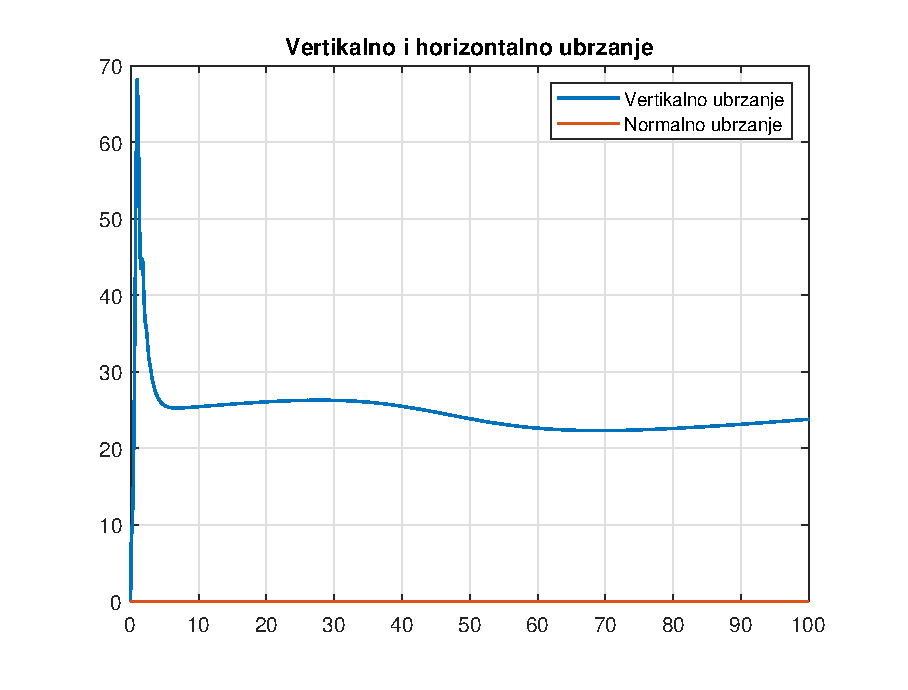
\includegraphics[scale= 0.5]{ubrVis.eps}
    \caption{Vertikalno i normalno ubrzanje projektila za jedinični otklon krmila visine}
    \label{fig:ubrVis}
\end{figure}
Sada se jasno vidi da se za jedinični otklon krmila visine postiže stalno vertikalno ubrzanje, što se slaže sa 
činjenicom da projektil čini kružnu putanju u $xz$ ravnini. Nulto horizontalno ubrzanje 
se slaže sa činjenicom da projektil ne čini pomjeraje u horiznotalnoj ravnini. 
Sada posmatrajmo odziv projektila za jedinični otklon krmila pravca. Ovdje će se izvršiti 
duža simulacija kako bi se dobila bolja analiza. Na slici \ref{fig:putanjePrav} su prikazane 
putanje u $xz$ i $xy$ ravninama kada se ima jedinični otklon krmila pravca projektila. 
\begin{figure}[!ht]
    \centering
    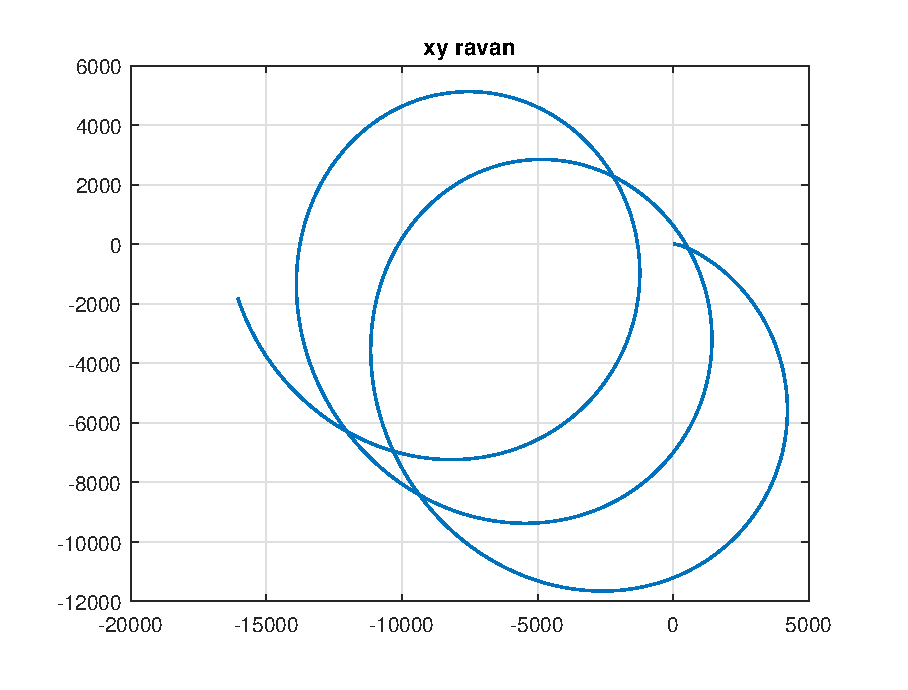
\includegraphics[scale=0.5]{xyPrav.eps}
    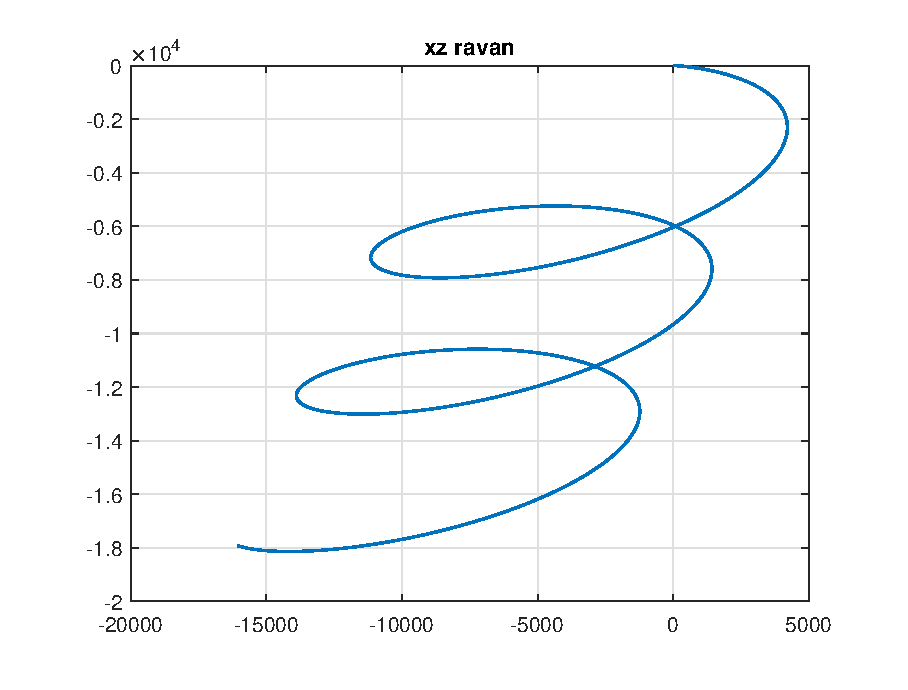
\includegraphics[scale=0.5]{xzPrav.eps}
    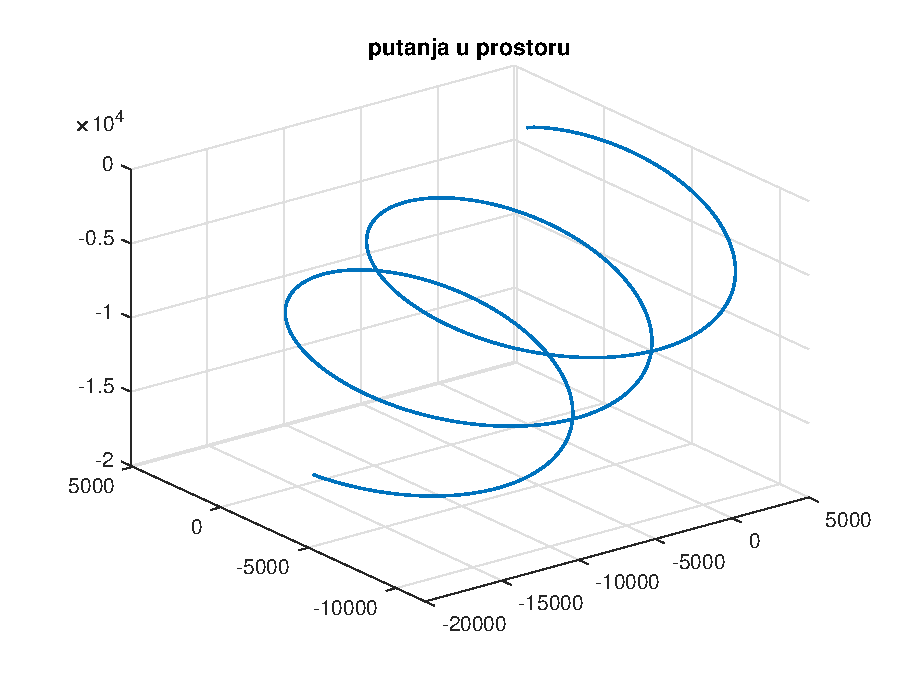
\includegraphics[scale=0.5]{3dprav.eps}
    \caption{Putanje pri jediničnom otklonu krmila pravca}
    \label{fig:putanjePrav}
\end{figure}
Sada se vidi da kada se zakrene krmilo visine, da projektil čini kružnu putanju u $xy$ ravni, što je bilo 
i očekivano. Naravno pomjeraj po $x$ osi mora da postoji zbog stalne sile potiska. Vidi se da u 
$xz$ ravnini, projektil pada na zemlju ali i treba primjetiti da se projektil u nekim 
trenutcima počinje dizati po $z$ osi. Ovo je posljedica postojanja pogonske sile i statičke stabilnosti projektila. 
Pošto je centar gravitacije projektila ispred centra pritiska, projektil se počne rotirati tako da mu nos 
pokazuje ka zemlji, međutim zbog otklona krmila visine on počne rotirati u oko svoje $z$ ose pa u jednom trenutku 
njegov nos bude okrenut suprotno od zemlje te zobg pogonske sile kratko započne kretanje ka gore sve dok se 
zobg otklona krmila pravca ne nastavi rotirati i posljedično nastavi smanjivati visinu. 
Promjene orijentacije projektila se vide na slici \ref{fig:eulerPravac}
\begin{figure}[!ht]
    \centering
    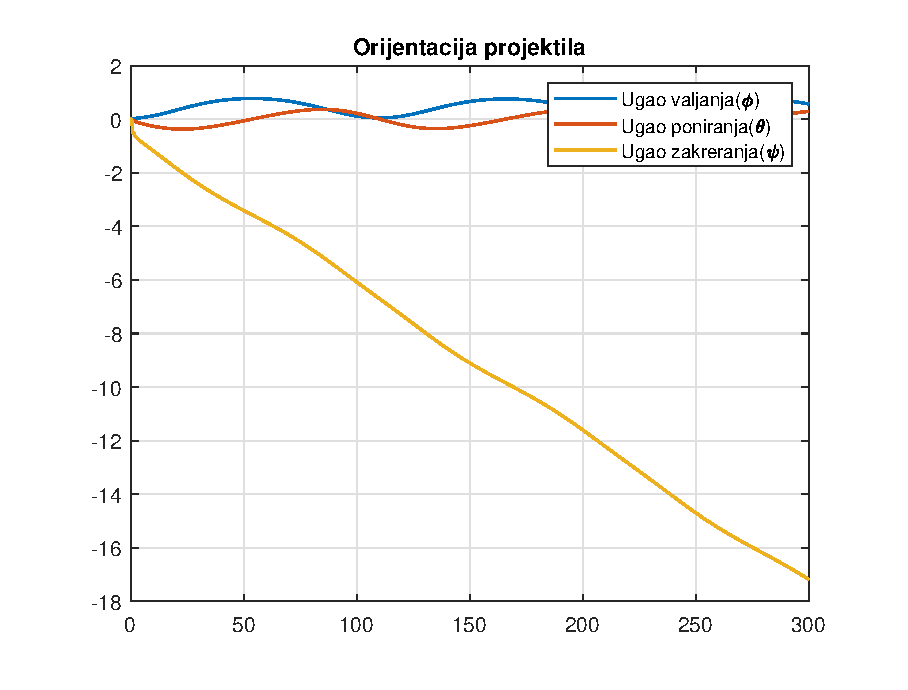
\includegraphics[scale = 0.5]{eulerPravac.eps}
    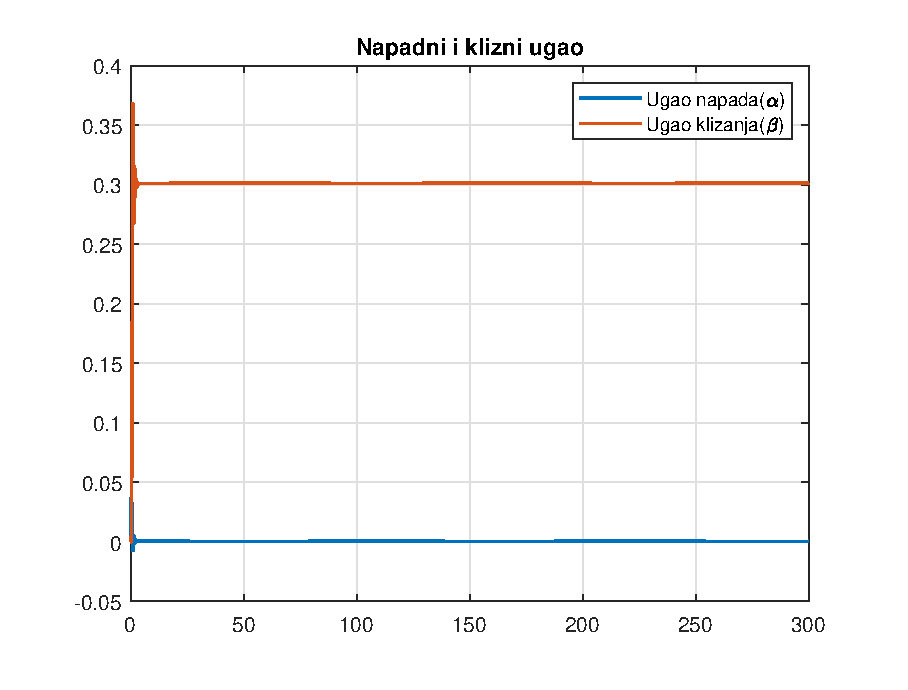
\includegraphics[scale = 0.5]{AOApravac.eps}
    \caption{Orijentacija projektila i ugao klizanja za jedinični otklon krmila pravca}
    \label{fig:eulerPravac}
\end{figure}
Vidi se na prethodnoj slici da ugao valjanja i ugao poniranja variraju, što objašnjava 
varijacije visine projektila i vidi se ugao zakretanja opada što objašnjava kružno kretanje 
u $xy$ ravnini. Posljedica toga je i konstantan ugao klizanja. Važno je istaći da je kanal pravca 
sistem neminimalne faze jer se za pozitav otklon krmila pravca, dobija negativan odziv ugla zakretanja. 
U nastavku se posmatra primjer horizontalnog hitca početnom brzinom od $100m/s$ u $x$ smjeru
sa visine $500m$. Kada ne bi bilo otpora vazduha i pogonske sile za očekivati je da će projektiil pasti na zemlju 
za $10.09$ sekundi. Naravno, zbog postojanja pogonske sile projektil će za nešto kraće vrijeme 
dotaknuti tlo. Pri ovoj simulaciji pretpostavljen je jedinični otklon elerona, pa će se pojaviti i valjanje. 
Na slici \ref{fig:eleronPutanja} su prikazane putanje kod ovog primjera. 
\begin{figure}[!ht]
    \centering
    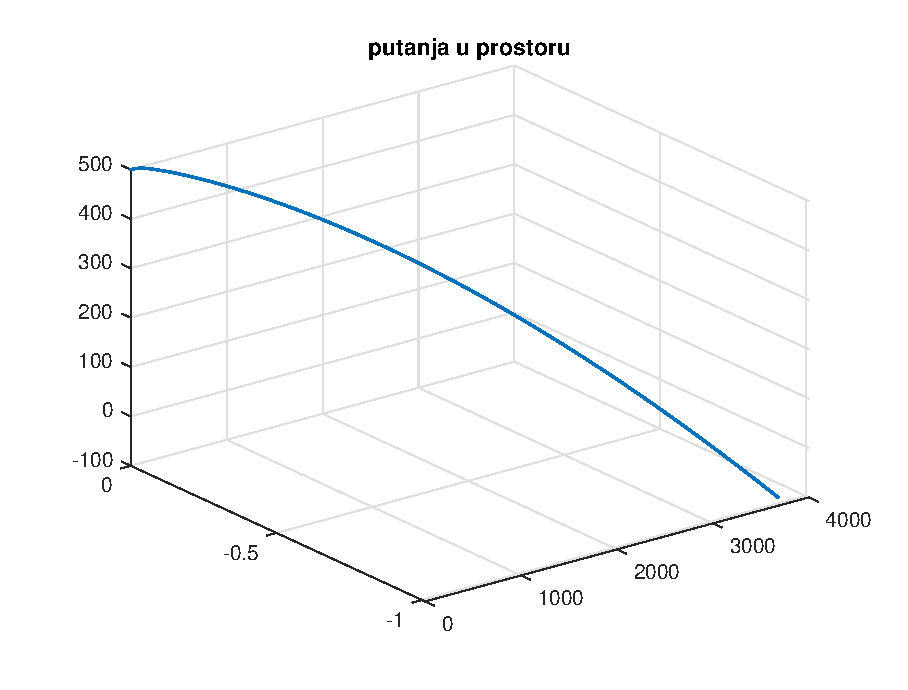
\includegraphics[scale = 0.7]{3deelron.eps}
    \caption{Trajekroija horizontalnog hitc sa jediničnim otklnom elerona}
    \label{fig:eleronPutanja}
\end{figure}
Vidi se da u ovom primjeru projektil, kao što je i očekivano, približno prati parabolu. 
Sada pogledajmo šta se dešava sa orijentacijom projektila. Na slici \ref{fig:orijentacijaEleron}
su prikazani Eulerovi uglovi. 
\begin{figure}[!ht]
    \centering
    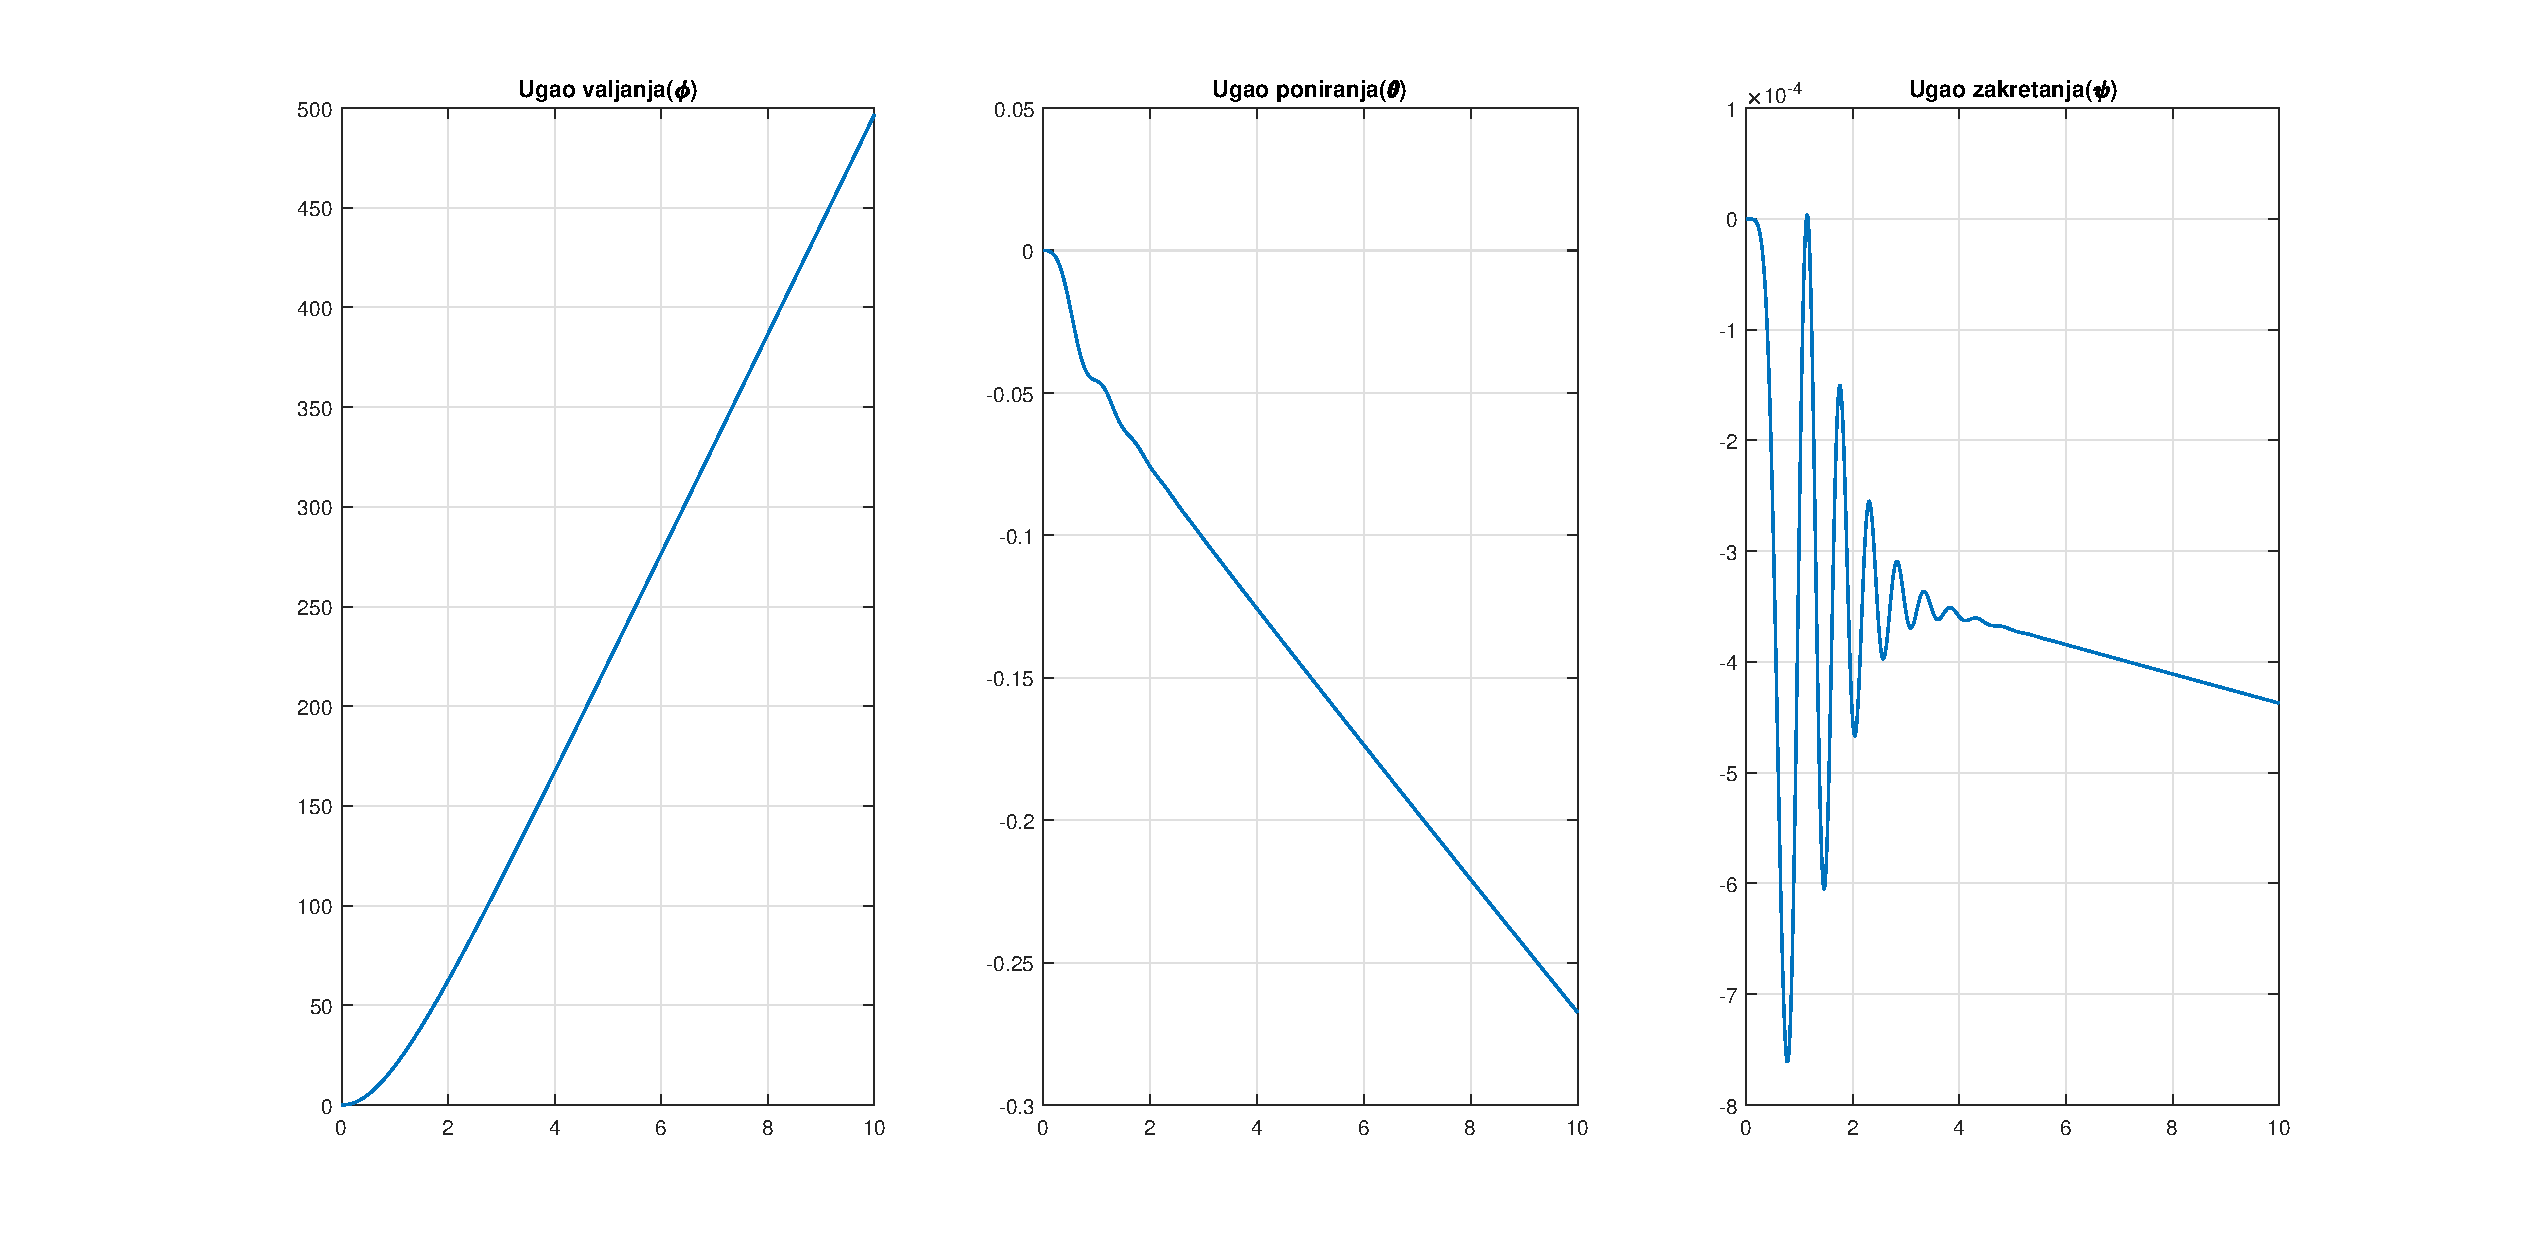
\includegraphics[scale = 0.4]{horHitacUglovi.eps}
    \caption{Orijentacija projektila pri horizontalnom hitcu sa jediničnim otklnom elerona}
    \label{fig:orijentacijaEleron}
\end{figure}
Zbog otklona elerona dolazi do porasta ugaone brzine valjanja što ima za posljedicu 
rast ugla valjanja. Prisjetimo se da se ugao valjanja ponaša kao čisti integrator i da je 
opisan diferencijalnom jednačinom:
\begin{equation*}
    \frac{dP}{dt} = L
\end{equation*}
Zbog ovoga za bilo kakvu promjenu otklona elerona, dolazi do rasta(po amplitudi) ugla valjanja. 
Promjena ugla propinjanja se može jednostavno objasniti pojavom uzgona. Pošto se centar pritiska nalazi 
iza centra gravitacije, javlja se moment koji zakreće projektil nadole. Kada bi simulacija duže trajala 
ugao propinjanja bi dosegao vrijednost skoro -90 stepeni. Posmatrajući treći grafik na kojem 
je prikazan ugao zakretanja vide se male promjene ugla zakretanaja(reda $10^{-4}$). U ovom primjeru,
bočno kretanje je zanemarljivo, ali ako postoje komponente brzine u sva tri smjera sistema tijela tada 
promjena brzine valjnanja može imati ozbiljne posljedice na stabilnost projektila i čak dovodi u pitnaje proces vođenja.
Za bolji uvid, na slici \ref{fig:eleronUbrzanja} su prikazani vertikalno i horizontalno ubrzanje projektila(poslije će se pokazati 
da su vertikalno i horizontalno ubrzanje presudni za proces vođenja).  
\begin{figure}[!ht]
    \centering
    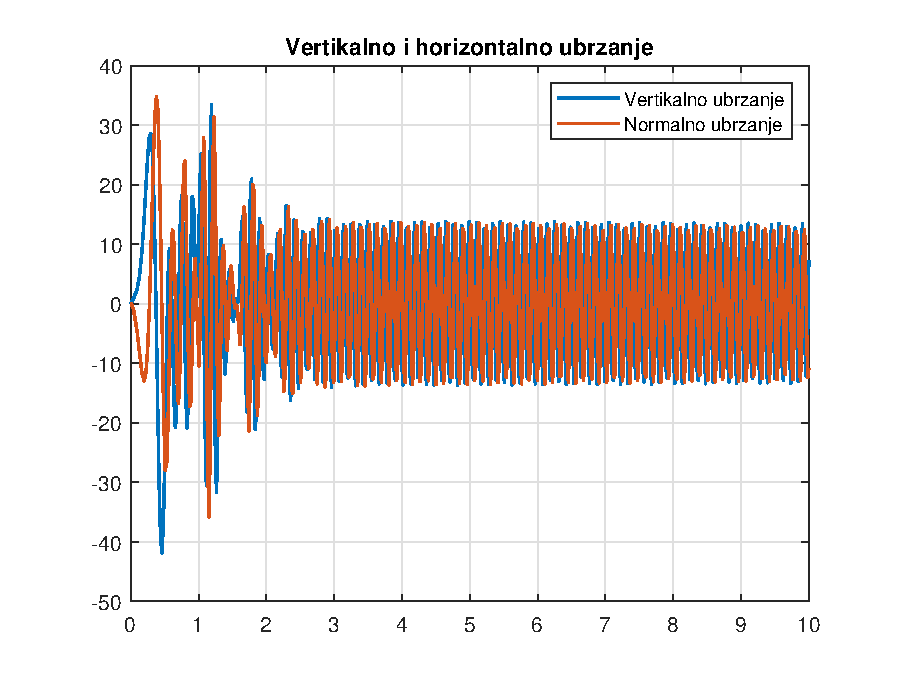
\includegraphics[scale=0.7]{eleronUbrzanja.eps}
    \caption{Vertikalno i normalno ubrzanje pri jediničnom otklonu elerona}
    \label{fig:eleronUbrzanja}
\end{figure}
Ovdje se vide velike oscilacije ubrzanja kada se pojavi kretanje u kanalu valjanja. Pošto se 
ova ubrzanja koriste kao referentna vrijednost kod vođenja projektila, neophodno je stabilizirati 
kanal valjanja kako bi se poboljšala regulacija ubrzanja. 
Dalje, pri velikim brzinama projektila i kretanju u kanalu valjanja dolazi do pojave couplinga 
kanala visine i kanala skretanja. Prema tome svi projektili krstaste konfiguracije 
kao prvi zahtjev pri dizajnu autopilota imaju stabilazaciju ugla valjanja. 
\section{Rasprezanje dinamičkog modela}
Sada će se u svrhu lakše analize i sinteze regulatora izvršiti rasprezanje dinamičkog modela. Ideja je 
da se uvedu neke pretpostavke koje će omogućiti da se predstavljene jednačine razdvoje na grupe 
nezavisnih jednačina.Treba da je ispunjeno:
\begin{itemize}
    \item Projektil se kreće u vertikalnoj ravni referentnog koordinatnog sistema.
    \item Osa $x_z$ leži u ravni kretnja.
\end{itemize}
Prva pretpostavka iziskuje $\beta , \phi , P, R\approx 0$. Činjenica da je $P,R \approx 0$ znači da se tijelo rotira samo oko $Y_b$ ose
,dalje, pretpostavka da je $\beta \approx 0$ znači da je usmjerenje letjelica isto kao i vektor brzine i konačno činjenica 
da je $\phi \approx 0$ znači da nema valjanja.  
Druga pretpostavka iziskuje $\Psi, \psi, y_z\approx 0$. Ovo znači da nema skretanja, da projektil može mjenjati samo visinu i udaljenost po $X_z$ osi.
Dakle ove dvije pretpostavke ograničavaju kretanje letjelice na vertikalnu ravan sa dopuštenjem propinjanja i kretanjem naprijed. 
Sada preostale jednačine koje su okarakterisane varijablama stanja:
\[V,\Theta,\theta,\alpha,Q,x_z, z_z\]
Definišu \textit{longitudinalno kretanje(kretanje u vertikalnoj ravni)}. Jednačine okarakterisan varijablama 
koje su u ovom slučaju zanemarene definišu \textit{lateralno kreetanje(bočno)} koje se sastoji 
od kretanja u horizntalnoj ravni, skretanja i valjanja ali bez propinjanja. Sada se ova dva podsistema mogu odvojeno posmatrati.
Sada ostaje samo da se sile koje su objašnjenje u prethodnom poglavlju pretvorimo iz sistema tijela 
i sistema Zemlje u sistem brzine i da ih se uvrsti u jednačine koje opisuju model u sistemu brzine. 
Jednačine koje predstavljaju longitdunalno kretanje su:
\begin{align}
    &m\frac{dV}{dt}= P\cos\alpha - R_{otp} - G\sin\Theta\\
    &mV\frac{d\Theta}{dt} = -Psin\alpha - R_{uzg} + G\cos\Theta\\
    &I_x\frac{dQ}{dt} \approx M\\
    &\frac{d\theta}{dt}=Q\\
    &\frac{dx_z}{dt}=V\cos\Theta\\
    &\frac{dz_z}{dt}=-V\sin\Theta
\end{align}
Također iz matrice transformacije $Tz^v$(treba invertovati $Tv^z$) se dobija za uvedene pretpostavke:
\begin{equation}
    \Theta = \theta - \alpha
\end{equation}
Sada se mogu napisati i jednačine za lateralno kretanje:
\begin{align}
    &mVcos\Theta \frac{d\Psi}{dt}=-P\cos\alpha \sin\beta \cos\phi - P\sin\alpha\sin\phi 
    - R_{side}\cos\phi - R_{uzg}\sin\phi\\
    &I_x\frac{dP}{dt}=L\\
    &I_z\frac{dR}{dt}=N+(I_x-I_y)\\
    &\frac{d\psi}{dt}=(R\cos\phi+q\sin\phi)/\cos\theta\\
    &\frac{d\theta}{dt}=P+(R\cos\phi - q\sin\phi)/\tan\theta\\
    &\frac{dy_z}{dt}=V\cos\Theta\sin\Psi
\end{align}
Pri čemu se iz $Tz^v$ pokazuje:
\begin{equation}
    \Psi \approx \psi-\beta
\end{equation}
Još uvijek se nisu u diferencijalne jednačine uvele linearizirane vrijednosti za aerodinamičke 
sile i momente pa se u jednačinama ne pojavljuju upralvjačke varijable, zbog toga će se u nastavku uraditi
poptuna linearizacija dinamičkog modela. Tada će se dobiti zavisnost varjiabli stanja od ulaza, pa 
je na osnovu toga moguće riješiti ove jednačine da bi se odredile varijable stanja. Iz ovoga slijedi i obrat 
tj. da se mogu odrediti otkloni upralvjačkih površina da bi se postigle željene vrijednosti varijabli stanja 
koje zahtjeva zakon voođenja. Naravno ovakav postupak je u otvorenoj petlji pa se zbog netačnosti modela 
preporučuje upravljanje u zatvorenoj povratnoj sprezi. 
\section{Linearizacija u okolini nominalne trajektorije}
Generalno, kada se priča o linearizaciji sistema, radi se o linearizaciji oko neke radne tačke. Ideja je 
da se diferencijalna jednačina u okolini te radne tačke predstavi linearnim segmentnom, te da 
nakon toga ona ima linearnu zavisnot od ulaznih parametara. Kod kretanja projektila umjesto pojma 
radne tačke se uvodi pojam \textit{nominalne trajektorije}. To je trajektorija po kojoj projektil 
leti kada su sve varijable stanja upravo onakve kako se od njih očekuje da budu i kada nema vanjskih poremećaja 
na projektil osim aerodinamičkog otpora i gravitacije. Sada se kao suprotnost nominalnoj trajektoriji 
uvodi pojam \textit{pormećajnog kretanja} koje se odlikuje odstupanjem varijabli stanja od nominalnih vrijednosti. 
Pri ovome se pretpostavlja da su odstupanja varijabli stanja pri poremećajnom kretanju relativno mala u odnosu na 
njihove nominalne vrijednosti. Svaka nominalna trajektorija određena je nekom vrijednošću vektora stanja $X_{nom}$.
Do ostalih vrijednosti može se doći rješavanjem jednačine:
\begin{equation}
    \dot{\vec{X}}_{nom} = f(\vec{X}_{nom}, \delta_{nom})
\end{equation}
Sada će se izvšiti linearizacija modela longitudinalnog kretanja. Pretpostavlja se da u okolini radne tačke, 
vrijednosti varijabli stanja imaju oblik:
\begin{equation}
    x=x_0+\Delta x 
\end{equation}
Prisjetimo se samo da u okolini nominalne trajektorije upravlja;ki signal može definisati kao:
\begin{equation}
    u(t) = u_0(t)+\Delta u(t)
\end{equation}
Pa je:
\begin{equation}
    \dot{x}_0(t)+\Delta \dot{x}(t)=f(x_0(t)+\Delta x(t),u_0(t)+\Delta u(t))
\end{equation}
Funkcija na desnoj strani se može raziti u Taylorov red i nakon odbacivanja članova višeg reda
se dobija:
\begin{equation}
    \dot{x}_0(t)+\Delta \dot{x}(t)=f(x_0(t),u_0(t))+\frac{\partial f}{\partial x}\Delta x+\frac{\partial f}{\partial u}\Delta u
\end{equation}
Sada se može napisati:
\begin{equation}
    \Delta \dot{x}(t)=\frac{\partial f}{\partial x}\Delta x+\frac{\partial f}{\partial u}\Delta u
\end{equation}
Parcijalni izvodi se uzimaju tako da vrijedi $x=x_0$ i $u=u_0$.\\
Kod modela longitudinalnog kretanja će se izvršiti isti postupak s tim da će se linearizirati svaka 
jednačina posebno. Sada za model longitduinalnog kretanja, ako se pretpostavi da se 
projektil kreće po nominalnoj trajektiri, vrijede jednačine:
\begin{align}
    &V=V_0+\Delta V \\
    & \alpha = \alpha _0+\Delta \alpha\\
    & \Theta=\Theta _0 +\Delta \Theta\\
    & \theta= \theta _0+\Delta \theta\\
    & Q=Q_0+\Delta Q\\
    & z_z=z_{z0}+\Delta z_z\\
    & \delta _V=\delta _{V0}+\Delta \delta _V
\end{align}
Koristeći pretpostavku da je $\cos\alpha_0 \approx 1$ i koristeći gore predstavljenu metodologiju 
linearizacije može se dobiti:
\begin{align}
    &\frac{d\Delta V}{dt}=\frac{P^V-F_o^V}{m}\Delta V - \frac{P\alpha+F_0^\alpha}{m}\Delta\alpha - g\cos\Theta _0\Delta\Theta +\frac{F_u^{\delta )V}}{m}\delta_V+\frac{X_P}{m}\\
    &\frac{d\Delta \Theta}{dt}=\frac{P^V-F_u^V}{m}\Delta V + \frac{P-F_u^\alpha}{mV}\Delta \alpha-\frac{g}{V}\sin\Theta\Delta\Theta-\frac{F_u^{\delta_V}}{\Delta_V}+\frac{Z_P}{mV}\\
    &\frac{d\Delta Q}{dt}=\frac{M^V}{I_y}\Delta V+\frac{M^\alpha}{I_y}\Delta Q+\frac{M^{\dot{\alpha}}}{I_y}\Delta\dot{\alpha}+\frac{M^{\delta_V}}{I_y}\Delta \delta_V+\frac{M^{\dot{\delta}_V}}{I_y}\Delta \dot{\delta}_V+\frac{M_P}{I_y} \\
    &\frac{d\Delta \theta}{dt}=\Delta Q \\
    &\frac{d\Delta x_z}{dt}=\cos\Theta_0\Delta V-V\sin\Theta_0\Delta\Theta\\
    &\frac{d\Delta z_z}{dt}=\sin\Theta_0\Delta V+V\cos\Theta_0\Delta\Theta \\
    &\Delta\alpha=\Delta\theta - \Delta\Theta
\end{align}
U koeficijentima dobijenih diferencijalnih jednačina su exponentima označeni izvodi te veličine. Konkretno, 
$P^V=\frac{\partial P}{\partial V}$, $F_o^\alpha = \frac{\partial F_o}{\partial \alpha} = QSC_o^\alpha$ etc. 
Svi ovi parcijalni izvodi su objašnjeni kada se govorilo o prirodi aerodinamičkih sila i momenata i oni se često 
za projektil daju tabelarno. Članovi $X_P$, $Z_P$ i $M_P$ predstavljaju poremećaje u vidu sila i momenata i oni ovdje 
djelom predstavljaju ulaze u sistem. Sada se u ovim jednačinama po prvi put eksplicitno vide upravljačke varijable.  
Na isti način se mogu naći i lineariziane jednačine za lateralno kretanje.
Ako se nađe Laplasova transformacija gornjih jednačina, rješavanjem dobijenog sistema algebarskih jednačina 
dobija se karakteristični polinom funkcija prenosa(sjetimo se da kod MIMO sistema, sve prenosne funkcije imaju isti karakteristični polinom). 
Radi se o polinomu četvrtog reda kod kojeg je jedan par polova po modulu dosta veći od drugog para polova po modulu. 
Sada je jasno da se kretanje letjelice može razdovjiti na \textit{brzo prigušeno} kretanje koje može biti oscilatorno 
ili aperiodičko i na \textit{fugoidno(sporo prigušeno)}. Dinamiku modela longitudinalnog kretanja određuje 
dominantni par polova koji je manji po modulu pa je kretanje letjelice određeno fugoidnim kretanje. Sada je jasno da se 
polovi koji opsiuju brzoprigušeno kretanje mogu odbaciti pa će karakterisični polinom imati samo dva pola. 
Dakle, sada se posmatraju samo jednačine koje opisuju kratkoperiodično kretanje. Brzoperiodično kretanje je 
određeno jednačinom promjene brzine(prva diferencijalna jednačina) pa se nakon uvođenja ove pretpostavke odbacuje ova 
jednačina  i u ostalim se anulira $\Delta V$. Sada teba primjetiti da se u lineariziranim jednačinama pojavljuje koeficijent 
$-\frac{g}{V}\sin\Theta_0$. Ovaj koeficijent predstavlja uticaj gravitacije na longitudinalno kretanje. Za male elevacione 
uglove, ovaj koeficijent je jako blizak nuli. Čak i kada trajektorija puno odstupa od horizontalne, brzina projektila 
je najmanje 20 puta veća od gravitacionog ubrzanja pa se uticaj gravitacije na longitudinalno kretanje može zanemariti. 
Ova pretpostavka u prenosnim funkcijama uvodi pol u nuli, tj. pod ovom pretpostavkom sistem će se ponašati kao integrator i 
sam će osiguratio nultu grešku stacionarnog stanja. Međutim ako ova pretpostavka nije ispunjenja tada će se pojaviti pol blizak nuli, 
pa će prelazni proces biti dug možda čak i nestabilan. Sada, pod ovim pretpostavkama dobijaju sljedeće prenosne funkcije:
\begin{align}
    &\frac{\Delta \theta(s)}{\Delta \delta_V(s)}=\frac{K(T_1s+1)}{s(T^2s^2+2\xi Ts+1)}\\
    &\frac{\Delta \Theta(s)}{\Delta \delta_V(s)}=\frac{K}{s(T^2s^2+2\xi Ts+1)}\\
    &\frac{\Delta \alpha(s)}{\Delta \delta_V(s)}=\frac{KT_1}{T^2s^2+2\xi Ts+1}\\
    &\frac{\Delta n_z(s)}{\Delta \delta_V(s)}=\frac{V}{g}\frac{K}{T^2s^2+2\xi Ts+1}
\end{align}
,gdje $n_z = \frac{V\dot{\Theta}}{g}$ predstavlja \textit{normalno preopterećenje}, tj. odnos ubrzanja koje je normalno na pravac brzine i gravitacione konstante. 
Evidentno je da je normalno ubrzanje definisano izrazom:
\begin{equation}
    a_z = V\dot{\Theta}
\end{equation}
I predstavlja jako bitnu veličinu jer mnogi zakoni vođenja generišu komandne signale u vidu normalnog ubrzanja projektil, pa će se i 
posebna pažnja posvetiti upravljanju normalnog ubrzanja. Prenosna funkcija koja određuje normalno ubrzanje je:
\begin{equation}
    \frac{\Delta a_z(s)}{\Delta \delta_V(s)} =\frac{KV}{T^2s^2+2\xi Ts+1}
\end{equation}
\begin{figure}[!ht]
    \centering
    \begin{tikzpicture}[auto, node distance=2cm,>=latex']
        \node[input, name=input](input){};
        \node[block, right of = input, node distance = 3cm] (g1){$\frac{KT_1}{T^2s^2+2\xi Ts+1}$};
        \node[block, right of = g1, node distance = 3cm] (g2) {$\frac{T_1s+1}{T_1s}$};
        \node[block, right of = g2] (g3){$\frac{1}{1+T_1s}$};
        \node[anchor = south] (alpha) at ($(g1)!0.6!(g2)$){$\alpha$};
        \node[anchor = south] (theta) at ($(g2)!0.5!(g3)$){$\theta$};
        \node [output, right of = g3] (output) {};
        \node[block, below of = g3] (g4) {$\frac{V}{gT_1}$};
        \node [output, right of = g4] (output2) {};
        \draw [->] (g3) -- node [name=y] {$\Theta$}(output);
        \draw[->] (g4)--node[] {$n_z$}(output2);
        \draw[->] (alpha)|-(g4);
        \draw [draw,->] (input) -- node {$\delta_V$} (g1);
        \draw[->](g1)--(g2);
        \draw[->](g2)--(g3);
\end{tikzpicture}
\caption{Blok dijagram lineariziranog modela longitudinalnog kretanja}
\label{fig:diagLongi}
\end{figure}
Evidentno je da za dobijanje lineariziranog modela longitudnalnog kretanja uvedeno 
puno pretpostavki i da će bilo kakvo odstupanje od ovih pretpostavki umanjiti vjerodostojnost modela, 
ali se pokazuje da je ovaj linearizirani model dosta dobra aproksimacija pri nominalnim uslovima leta. 


\chapter{Uvod u proporcionalnu navigaciju}
\section{Opis planarnog susreta}
\begin{figure}[!ht]
    \centering
    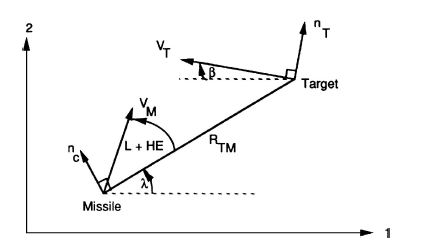
\includegraphics{PNfigure.JPG}
\end{figure}
\noindent Udaljenost između mete i projektila u svakom trenutku je data sa:
\begin{equation}
    r(t)=r_T(t)-r_M(t)
\end{equation}
Brzina približavanja projektila meti je data sa: 
\begin{equation}
    v_{cl}=-\dot{r}(t)
\end{equation}
Ugaono ubrzanje mete je dato sa:
\begin{equation}
    \dot{\beta}=\frac{n_T}{v_T}
\end{equation}
Kompnente vektora brzine mete u koordinatnom sistemu vezanom za zemlju su date sa:
\begin{equation}
    v_{T1}=-v_T\cos{\beta}
\end{equation}
\begin{equation}
    v_{T2}=v_T\sin{\beta}
\end{equation}
Slično tome, brzina i ubrzanje projektila su date sa:
\begin{equation}
    \dot{v}_{M1}=a_{M1}
\end{equation}
\begin{equation}
    \dot{v}_{M2}=a_{M2}
\end{equation}
\begin{equation}
    \dot{R}_{M1}=v_{M1}
\end{equation}
\begin{equation}
    \dot{R}_{M2}=v_{M2}
\end{equation}
Ugao \textit{Line of sight} se može izračunati kao:
\begin{equation}
    \lambda = \arctan{\frac{R_{TM2}}{R_{TM1}}}
\end{equation}
Pa je: 
\begin{equation}
    \dot{\lambda}=\frac{R_{TM1}v_{TM2}-R_{TM2}v_{TM1}}{r^2}
\end{equation}
Ugao između vektora pozicije i vektora brzine je dat sa:
\begin{equation}
    L=\arcsin{\frac{v_T\sin{(\beta+\lambda)}}{v_M}}
\end{equation}
Također treba uzeti u obzir da je:
\begin{equation}
    v_{cl}=-\dot{r}=v_M\cos\delta - v_T\cos\theta
\end{equation}
Te da će doći do sudara samo u slučaju da vrijedi: 
\begin{equation}
    v_M\cos\delta > v_T\cos\theta
\end{equation}
Upravljački zakon proporcionalne navigacije je dat sa:
\begin{equation}
    n_C=N'v_c\dot{\lambda}
\end{equation}

%-----------------------------
\section{Izvođenje upravljačkog zakona}
\begin{equation}
    \sin{\lambda}=\frac{y}{r}
\end{equation}
Za male uglove može se koristiti aproksimacija:
\begin{equation}
    \lambda \approx \frac{y}{r}
\end{equation}
, pa je:
\begin{equation}
    \dot{\lambda}(t)=\frac{\dot{y}(t)r(t)-y(t)\dot{r}(t)}{r^2}
\end{equation}
\begin{equation}
    \ddot{\lambda}(t)=\frac{\ddot{y}(t)-2\dot{\lambda}(t)\dot{r}(t)-\lambda(t)\ddot{r}(t)}{r(t)}
\end{equation}
Uvedimo vremenski varijantne koeficijente:
\begin{equation}
    a_1(t)=\frac{\ddot{r}(t)}{r(t)}
\end{equation}
\begin{equation}
    a_2(t)=2\frac{\dot{r}(t)}{r(t)}
\end{equation}
\begin{equation}
    b(t)=\frac{1}{r(t)}
\end{equation}
Pa se dobija diferencijalna jednačina drugog reda sa varijabilnim koeficijenitma:
\begin{equation}
    \ddot{\lambda}(t)=-a_1(t)\lambda-a_2(t)\dot{\lambda}+b(t)\ddot{y}(t)
\end{equation}
Uzimajući u obzir dobija se:
\begin{equation}
    \ddot{y}(t)=-a_M(t)+a_T(t)
\end{equation}
\begin{equation}
    \ddot{\lambda}(t)=-a_1(t)\lambda-a_2(t)\dot{\lambda}-b(t)a_M(t)+b(t)a_T(t)
\end{equation}
Neka je $x_1(t)=\lambda$ i $x_2(t)=\dot{\lambda}$. Tada je susret projektila i mete opisan sljdećim diferencijalnim jednačinama prvog reda.
\begin{equation}
    \dot{x}_1=x_2
    \label{eq:1}
\end{equation}
\begin{equation}
    \dot{x}_2=-a_1(t)x_1-a_2(t)x_2-b(t)u+b(t)f
    \label{eq:2}
\end{equation}
,gdje je uzeto $u=a_M(t)$ i vanjska smetnja $f=a_T(t)$.
Prvo posmatrajmo slučaj kada meta ne ubrzava, tj. kada je $f=0$. Sada se problem proporcionalne navigacije može predstaviti kao:
\begin{tcolorbox}
    Pronaći upravljački signal $u$ tako da je sistem opisan jednačinama \ref{eq:1} i \ref{eq:2} asimptotski stabilan u odnosu na $x_2$
\end{tcolorbox}
Shodno tome, uzmimo Lyapunovu funkciju $Q$:
\begin{equation}
    Q=\frac{1}{2}cx_2^2
\end{equation}
Izvod po vremenu duž bilo koje trajektorije je:
\begin{equation}
    \dot{Q}=cx_2(-a_1(t)x_1-a_2(t)x_2-b(t)u(t))
\end{equation}
Sada se vidi da upravljački signal 
\begin{equation}
    u=kx_2=k\dot{\lambda}
    \label{eq:3}
\end{equation}
Stabilizuje sistem dat sa \ref{eq:1} i \ref{eq:2} ako $k$ zadovoljava:
\begin{equation}
    kb(t)+a_2(t)>0
\end{equation}
,odnosno \begin{equation}
    k>-2\dot{r}(t)=2v_{cl}
\end{equation}
Prema tome, uvodeći \textit{efektivni navigacijski odnos} $N$, izraz \ref{eq:3} postaje:
\begin{equation}
    u=Nv_{cl}\dot{\lambda}(t) \quad ,N>2
\end{equation}
čime je potpuno određen zakon vođenja proporcionalne navigacije.
Za trodimenzionalni slučaj se bira kandidat funkcija:
\begin{equation}
    Q=\frac{1}{2}\sum_{s=1}^3d_s\dot{\lambda}_s^2
\end{equation}
, gdje su $d_s$ pozitivni koeficijenti. Analogno se dobija upravljački zakon:
\begin{equation}
    u_s=Nv_{cl}\dot{\lambda}_s \quad ,N>2\ (s=1,2,3)
\end{equation}
\section{Izmjenjena proporcionalna navigacija}
Za mete koje manevrišu i imaju neko normalno ubrzanje, za planarni sustre, izvod Lyapunove kandidat 
funkcije je:
\begin{equation}
    \dot{Q}=cx_2(-a_1(t)x_1-a_2(t)x_2-b(t)u(t)+b(t)f)
\end{equation}
Odakle se zaključuje da je upravljaki signal koji stabilizuje sistem:
\begin{equation}
    u=Nv_{cl}\dot{\lambda}(t)+\frac{N}{2}a_T(t) \quad ,N>2
\end{equation}
\section{Optimalnost zakona proporcionalne navigacije}
Ako je promjena LOS ugla različita od nule, tada se primjenjuje normalno ubrzanje kako bi 
se promjena svela na nulu. U prethodnoj sekciji se proporcionalna navigacija predstavila kao 
problem upravljanja gdje je normalno ubrzanje bilo upravljački signal, a brzina promjene LOS ugla bila varijabla stanja.
Proporcionalna navigacija se može posmatrati kao problem optimalnog upravljanja. Treba pronaći indeks performansi koji 
proporcionalna navigacija minimizira. Ovo predstavlja inverzni problem problem optimalnog upravljanja. Pretpostavimo da 
se projektil približava meti konstantnom brzinom. Ignorišuči dinamiku projektila, vrijedi:
\begin{equation}
    \ddot{y}=-a_M,\ y=r\lambda,\ r(\tau)=v_{cl}\tau
\end{equation}
Također pretpostavlja se da nema kašnjenja u dinamici projektila, tj. da je $a_M = a_{M_c}$.
Definišimo sada ineks performansi:
\begin{equation}
    J=\frac{1}{2}Cy^2(t_f)+\frac{1}{2}\int_0^{t_f}{a_M^2dt}
\end{equation}
Prvi član predstavlja promašaj(miss distance), a drugi predstavlja energiju energiju utrošenu u toku leta. Ideja je pronaći upravljanje
$a_M$ koje minimizira kriterij performanse $J$. Koriteći Bellman-Lyapunov pristup dobija se da je 
optimalno upravljanje dato sa:
\begin{equation}
    a_M(t)=\frac{3\tau}{3/C+\tau ^3}(y(t)+\dot{y}(t)\tau)
\end{equation}
Nulti promašaj se dobija za $C\rightarrow \infty$, pa je optimalno upravljanje dato sa:
\begin{equation}
    a_M(t)=\frac{3}{\tau ^2}(y(t)+\dot{y}(t)\tau)
\end{equation}
Uzimajući u obzir da je:
\begin{equation}
    \dot{\lambda} = \frac{\dot{y}(t)r(t)-y(t)\dot{t}(t)}{r^2}=\frac{\dot{y}(t)\tau + y(t)}{r}
\end{equation}
jer je, $r=v_{cl}\tau$, dobija se:
\begin{equation}
    a_M(t)=3v_{cl}\dot{\lambda}
\end{equation}
Ovo znači da pod uvedenim pretpostavkama, proporcionalna navigacija minimizira kriterij performanse
$J$ i izbor efektivnog navigacijskog odnosa $N=3$ garantuje da nulti promašaj. 
%-----------------------
\section{Linearizacija}
\begin{figure}[!ht]
    \centering
    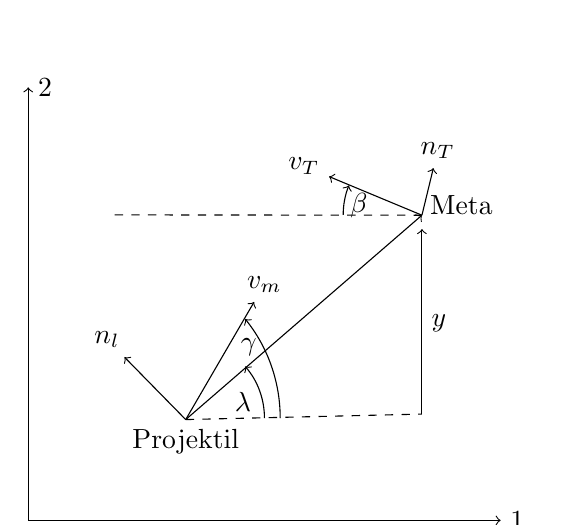
\begin{tikzpicture}
        \draw [->](0,0)--(0,5.5) node[right]{$2$};
        \draw [->](0,0)--(6,0) node[right]{$1$};
        \node[] at (2,1) (m){Projektil};
        \node[] at (5,4) (t){};
        \node[right of = t, node distance =0.5cm] (){Meta};
        \draw[->] (m.north) -- (t.south);
        \node[]at(3,3)(vm){$v_m$};
        \draw[->](m.north)--(vm);
        \node[] at (1,2.3) (nl){$n_l$};
        \draw[->] (m.north)--(nl);
        \draw[dashed] (m.north) -- (5,1.35);
        \node[anchor = west] at (2.5, 1.5) () {$\lambda$};
        \draw[->] (3,1.3) arc (0:41:1);
       \draw[->](3.2,1.3) arc (0:39:2);
       \node[] at (2.8, 2.2) () {$\gamma$};
       \draw[dashed] (t.south) -- (1,3.88);
       \node[] at (3.5,4.5)(vt){$v_T$};
       \draw[->] (t.south) -- (vt);
       \node[] at (5.2, 4.7) (nt){$n_T$};
       \draw[->](t.south) -- (nt);
       \draw[->] (5,1.35)--(5,3.7);
       \node[anchor = west] at (5, 2.5) (){$y$};
       \draw[->] (4, 3.88) arc (180:158:1);
       \node[] at (4.2,4) (){$\beta$};
\end{tikzpicture}   
    \caption{Linearizacija jednačina proporcionalne navigacije}
    \label{fig:linear}
\end{figure}
\noindent Linearizacija se može lahko izvršiti ako se definišu nove veličine koje su prikazane na slici \ref{fig:linear}.
Relativno ubrzanje se može odrediti sa slike i iznosi:
\begin{equation}
    \ddot{y}=n_T\cos\beta-n_c\cos\lambda
\end{equation}
Ako su uglovi leta mali, tada vrijedi:
\begin{equation}
    \ddot{y}=n_T-n_c
\end{equation}
Slično tako vrijedi:
\begin{equation}
    \lambda = \frac{y}{r}
\end{equation}
Za čeoni slučaj vrijedi:
\begin{equation}
    v_{cl}=v_M+v_t
\end{equation}
Za potjeru vrijedi:
\begin{equation}
    v_{cl}=v_M-v_t
\end{equation}
Sada se može linearizirati i jednačina za udaljenost:
\begin{equation}
    r(t)=v_{cl}(t_F-t)
\end{equation}
gdje je $t_F$ ukupno vrijeme leta.\\
Definišimo i veličinu \textit{time to go} $t_{go}$:
\begin{equation}
    t_{go}=t_F-t
\end{equation}
Linearizirani promašaj se definisše kao udaljenost mete i projektila na kraju leta, ili:
\begin{equation}
    Miss=y(t_f)
\end{equation}
\section{Petlja navođenja i zero effort miss}
Ranije je pokazano da vrijedi:
\begin{equation}
    \dot{\lambda}(t)=\frac{\dot{y}(t)r(t)+y(t)v_{cl}}{r^2}
\end{equation}
Kako vrijedi $r=v_{cl}t_{go}$, tada se dobija:
\begin{equation}
    \dot{\lambda}(t)=\frac{\dot{y}(t)t_{go}+y(t)}{v_{cl}t_{go}^2}
\end{equation}
Definišimo sada veličinu \textit{Zero effort miss}, koja predstavlja buduće relativno rastojanje projektila i mete:
\begin{equation}
    ZEM=\dot{y}(t)t_{go}+y(t)
\end{equation}
pa se dobija:
\begin{equation}
    \dot{\lambda}(t)=\frac{ZEM}{v_{cl}t_{go}^2}
\end{equation}
Ako se pretpstavi da će se pod uticajem ubrzanja $a_c$ postići sudar, $ZEM$ se može smatrati 
budućom tačkom susreta, pa se zakon vođenja proprcionalne navigacije može iskazati kao:
\begin{equation}
    a_c(t)=N\frac{ZEM}{t_{go}^2}
\end{equation}
Sada se vidi da je normalno ubrzanje projektila direktno proprorcionalnu $ZEM$-u i inverzno proporcionalno
kvadratu preostalom vremenu leta, što znači da se generiše veće ubrzanje što je susret bliži.
Pošto se $ZEM$ posmatra kao buduća tačka susreta, koja se računa na osnovu znanja ili pretpostavki 
budučeg kretanja mete, PN vođenje se smatra prediktivnim. $ZEM$ je koristan jer se može izračunati 
mnoštvom metoda uključujući i on-line numeričku integraciju nelinearnih diferencijalnih jednačina projektila 
i mete. Pretohdno izvedene linaerizovane jednačine proporcionalne navigacije se mogu 
prikazati blok dijagramom kao na slici \ref{fig:homing}.
\begin{figure}[htp]
    \centering
    \begin{tikzpicture}[auto, node distance=2cm]
        \node[input, name = nt] (nt){$n_T$};
        \node[sum, right of = nt, node distance=1cm](sum){};
        \node[block, right of = sum] (int2){$\frac{1}{s^2}$};
        \node[block, right of = int2] (div) {$\frac{1}{v_{cl}(t_f-t)}$};
        \node[block, right of=div](seeker){$s$};
        \node[block, below of = div](law){$Nv_{cl}$};
        \node[block, left of = law](dyn){$\frac{1}{1+T_ms}$};
        \node [output, right of=seeker, node distance=1cm] (output) {};
        \node (a) at ($(int2)!0.5!(div)$){};
        \node (miss) at ($(a) -(0, 0.145cm) $){};
        \node[above of = miss, node distance=1.5cm] (missArr){Promašaj};
        \draw[->] (miss)--(missArr);
        \node at (nt) [anchor = south ](){$n_T$};
        \node[left of = dyn, node distance = 1cm, anchor = south] () {$n_L$};
        \node[anchor = south] () at ($(dyn)!0.5!(law)$) {$n_C$};
        \node[right of = seeker,anchor = south, node distance = 1 cm] () {$\dot{\lambda}$}; 
        \draw[->](nt)--node[pos=0.95] {$+$}(sum);
        \draw[->](sum)--(int2);
        \draw[->](int2)--(div);
        \draw[->](div)--(seeker);
        \draw[->](output)|-(law);
        \draw[->](law)--(dyn);
        \draw [-] (seeker) -- node [name=y] {}(output);
        
        \draw[->](dyn)-|node[pos=0.99] {$-$}(sum);
        
        \end{tikzpicture}
    \caption{Petlja navođenja}
    \label{fig:homing}
\end{figure}
Ulaz sistema je ubrzanje mete, a u 
povratnoj sprezi se nalazi upralvjački zakon. Pretpostavlja se da je model trekera idealni diferencijator i sistem 
za navođenje ne uvodi nikakvo kašnjenje. U stvarnosti, sistem za navođenje se modelira prenosnom 
funkcijom prvog reda, tj:
\begin{equation}
    \frac{n_L}{n_c}=\frac{1}{1+sT}
\end{equation}
,gdje je $n_L$ ostvareno ubrzanje projektila, a $n_c$ zahtjevano ubrzanje projektila.
\begin{figure}[!ht]
    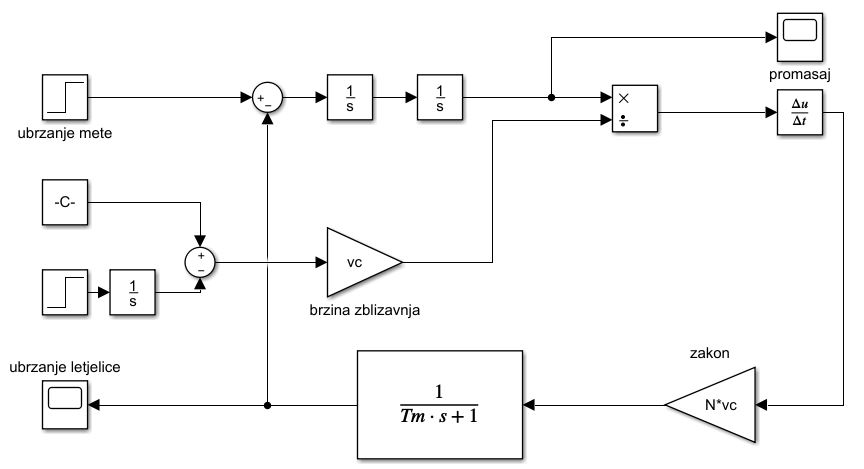
\includegraphics[scale = 0.6]{homingSimulink.JPG}
    \caption{Proporcionalana navigacija u Simulinku}
    \label{fig:simProp}
\end{figure}
Koristeći Simulink dijagram sa slike \ref{fig:simProp} izvršene su simulacije za $N=4$ i $N=5$
pri ubrzanju mete od $3g$. Ubrzanja projektila su prikazana na grafu \ref{fig:propAcc}.
\begin{figure}[htp!]
    \centering
    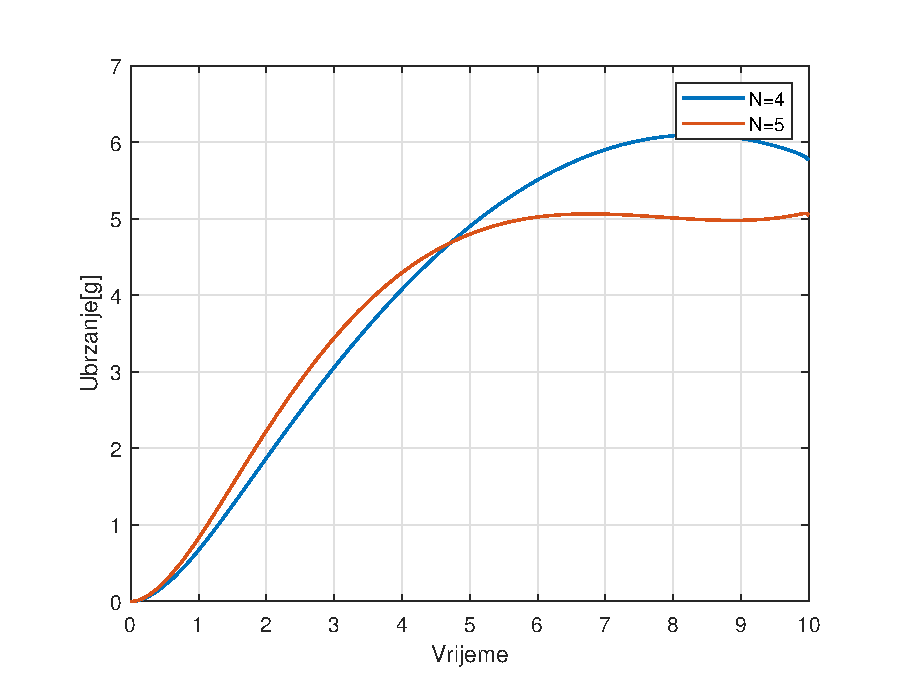
\includegraphics[scale = 0.5]{propAccPlot.eps}
    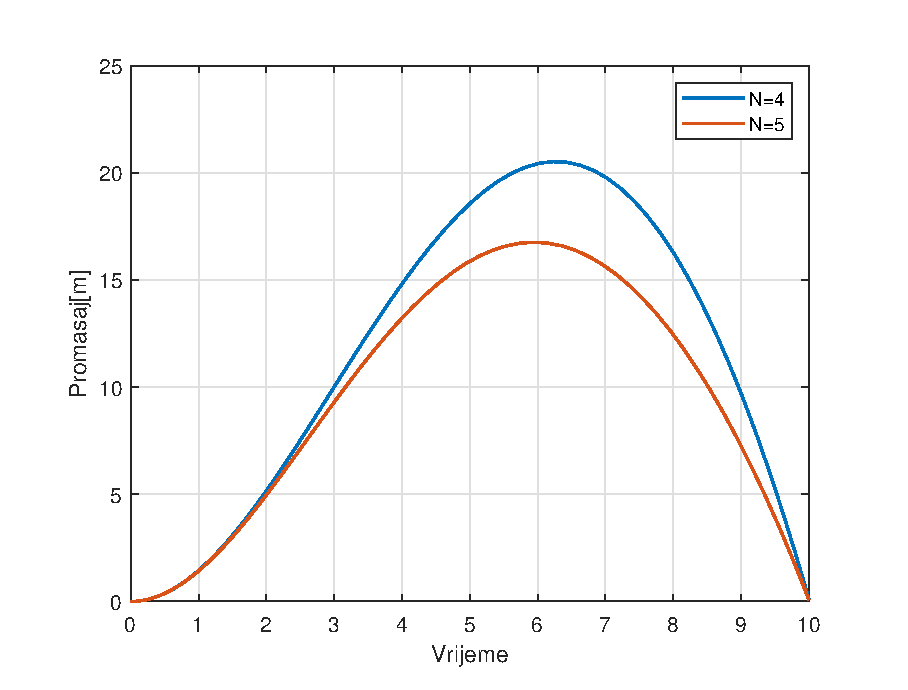
\includegraphics[scale = 0.5]{missProp.eps}
    \caption{Ubrzanja projektila i promašaj za $N=4$ i $N=5$}
    \label{fig:propAcc}
\end{figure}
Vidi se da veći efektivni navigacijski odnos zahtjeva manje ubrzanje projektila pa su time 
smanjeni i zahtjevi za performanasam projektila, međutim veći efektivni navigacijski odnos 
daje manji promašaj što se vidi na grafiku za promašaj na slici \ref{fig:propAcc}. 
U oba slučaja ostvaren je sudar unutar deset sekundi. U nastavku je na slici \ref{fig:simAugProp} prikazan 
simulink model izmjenjene proporcionalne navigacije.
\begin{figure}[!ht]
    \centering
    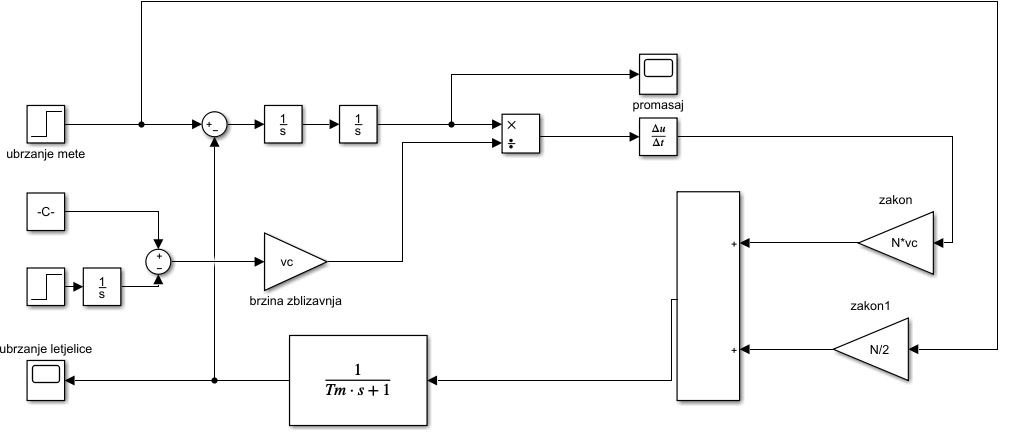
\includegraphics[scale = 0.6]{augPropSim.JPG}
    \caption{Simulink model izmjenjene proporcionalne navigacije}
    \label{fig:simAugProp}
\end{figure}
Ubrzanje projektila i promašaj su prikazana na graficima na slici \ref{fig:augPropGraf}.
\begin{figure}[!ht]
    \centering
    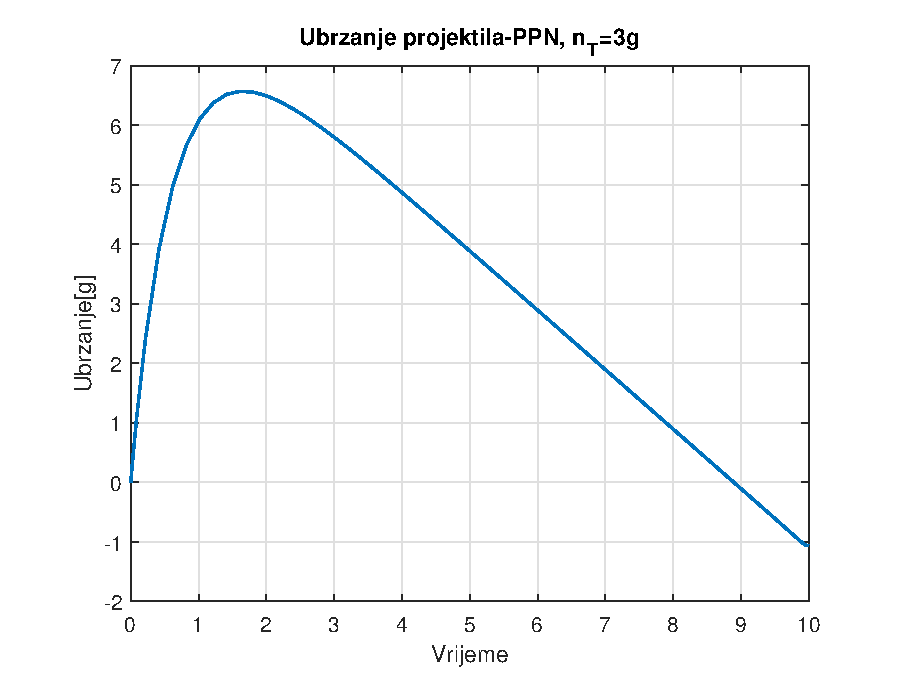
\includegraphics[scale = 0.5]{augPropAcc.eps}
    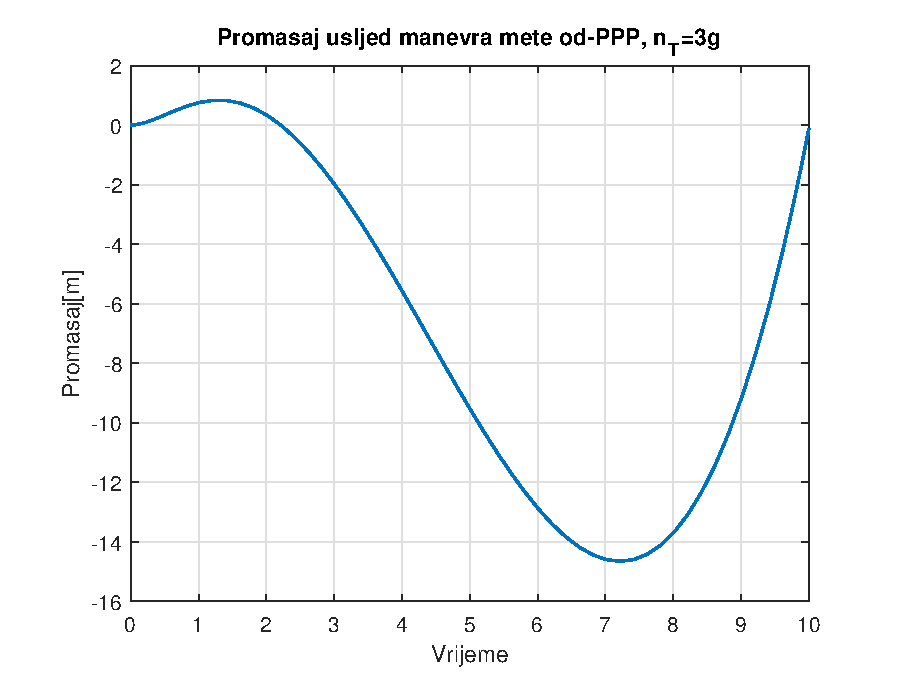
\includegraphics[scale = 0.5]{augPropMiss.eps}
    \caption{Ubrzanje projektila i promašaj vođen promjenjenom proporcionalnom naivgacijom, $N=3$}
    \label{fig:augPropGraf}
\end{figure}
Sada se konačno vidi da i kod proporcionalne navigacije i kod promjenjene proporcionalne navigacije 
se grantuje sudar unutar vrmena leta ako se izabere $N=3$. Dalje se vidi da 
ubrzanje projektila kod promjenjene proporcionalne navigacije počinje od nula za razliku od čiste proporcionalne 
navigacije. Kod promjenjene proporcionalne navigacije promašaj može postati negativan što iziskuje 
promjenu smjera normalnog ubrzanja projektila. 
\section{Adjungovani sistem i petlja navođenja}
Direktna simulacija lineariziranih jednačina proporcionalne navigacije se uvijek može
koristiti za generisanje upravljačkog signala(tj. normalnog ubrzanja) projektila
ali je tehnika nazvana \textit{adjungovana tehnika} historijski bila glavni računarski 
alat za dizajn i analizu vođenih projektila. Adjungovana tehnika je zasnovana 
na impulsnom odzivu sistema i koristi se  za analizu LTI sistema kao što je 
petlja navođenja projektila. Koristeći ovu tehniku mogu se dobiti tačne vrijednosti 
bilo koje veličine u datom trenutku.\\
Poznato je da je odziv sistema na prooizvoljni ulaz potpuno određen impulsnim odzivom sistema, pa 
tj. vrijedi da je odziv linearnog sistema dat sa:
\begin{equation}
    y(t)=\int_o^tu(\tau)h(t,\tau)d\tau
\end{equation}
Fizikalno, impuslni odziv $h(t-\tau)$ predstavlja odziv sistema na impulsnu pobudu koja 
se primjeni na sistem u trenutku $\tau$. Prema tome određivanje odziva sistema zahtjeva analitičku 
formu impulsnog odziva. Svaki linearni sistem ima i svoj adjungovani sistem i veza između impulsnog 
odziva linearnog sistema i njegovog adjungovanog sistema je data sa:
\begin{equation}
    h^*(t_f-\tau,t_f-t)=h(t,\tau)
\end{equation}
Ako se uzme da je ulaz sistema Heavysideov impuls, tada je odziv sistema dat sa:
\begin{equation}
    y(t)=a\int_0^t h^*(t_f-\tau,t_f-t)d\tau
\end{equation}
,nakon uvođenja smjene $x=t_f-\tau$, dobija se:
\begin{equation}
    y(t)=a\int_{t_f-t}^{t_f}h^*(x,t_f-t)dx
\end{equation}
Pošto je veličina od interesa promašaj na kraju leta uzima se $t_f=t$, pa prethodna relacija
postaje:
\begin{equation}
    y(t_f)=a\int_{0}^{t_f}h^*(x,0)dx
\end{equation}
Vidi se da se integracija vrši po posmatranom vremenu i da ne zavisi od trenutka primjene impulsa na adjunogvani sistem. 
Ovo znači da se izlaz u trenutku $t_f$ može dobiti primjenjujući impuls u početnom trenutku, te zatim integrišući ulaz. 
Konstrukcija adjungovanog modela se vrši prema naredna tri koraka:
\begin{enumerate}
    \item Pretvoriti sve ulaze sistema u impulse
    \item Zamjeniti $t$ sa $t_f-t$ i obratno na mjestima gdje se vrijeme pojavljuje kao argument
    \item Promjeniti smjer toka svih signala, mjenjajući sume sa čvorovima i obratno
\end{enumerate}
Koristeći navedena pravila dobija se adjungovana petlja navođenja prikazana na slici \ref{fig:adjHoming}, s tim 
da je kao smetnja u sistem dodata još i početna greška nišanjenja data sa $v_Me_q$ ,za $v_M=610\frac{m}{s}$ i $e_q=20\deg$.
Sada je moguće dobiti promašaj usljed manevra mete i promašaj usljed početne greške nišanjenja sve u jednoj 
simulaciji!
\begin{figure}[!ht]
    \centering
    \begin{tikzpicture}[auto, node distance=2cm,>=latex']
        \node[block] (nt) {$n_T$};
        \node[block, right of = nt](int1){$\frac{1}{s}$};
        \node[right of = int1] (center){};
        \node[block, right of = center](int2){$\frac{1}{s^2}$};
        \node[sum, right of = int2, node distance = 2cm](sum){+};
        \node[block, right of = sum](div){$\frac{1}{v_{cl}t}$};
        \node[block, below of = int2](law){$-\frac{N'v_{cl}s}{1+sT_m}$};
        \node[name = delta, above of = sum, node distance = 1.5cm](delta){$\delta(0)$};
        \node[left of = nt](out){Promašaj};
        \node[below of = out, node distance=0.3cm](out2){usljed};
        \node[below of = out2, node distance=0.3cm](){manevra mete};
        \node[right of = div](a){};
        \node at (center) [anchor = south west]{$\dot{x}_1$};
        \node[block, above of = center,node distance = 1.5cm](head){$-v_Me_q$};
        \node[above of = head, node distance = 1.5cm](m){};
        \node[right of = m, node distance =1cm](q){Promašaj};
        \node[below of = q, node distance = 0.3cm](w){usljed};
        \node[below of = w, node distance = 0.3cm](e){greške};
        \node[right of =e , node distance = 1.5cm](){nišanjenja};
        \draw[->](head)--(m);
        \draw[->](center.south)-- ++(0,0.1)--(head);
        \draw[->](delta)--(sum);
        \draw[->](sum)--(int2);
        \draw[->](int1)--(nt);
        \draw[->](div)--(sum);
        \draw[->](int2)--(int1);
        \draw[->](center.south)-- ++(0,0.13)|-(law);
        \draw[-](law)-|(a.east) -- ++(0,0.0215);
        \draw[->](a.east)-- ++(0.0215,0)--(div);
        \draw[->](nt)--(out);
        \end{tikzpicture}
    \caption{Adjungovana petlja navođenja}
    \label{fig:adjHoming}
\end{figure}
Jedinični impuls se može predstaviti kao početni uslov kod prvog integratora. Na slici \ref{fig:simAdj} 
je predstavljen Simulink dijagram adjungovanog sistema.
\begin{figure}[!ht]
    \centering
    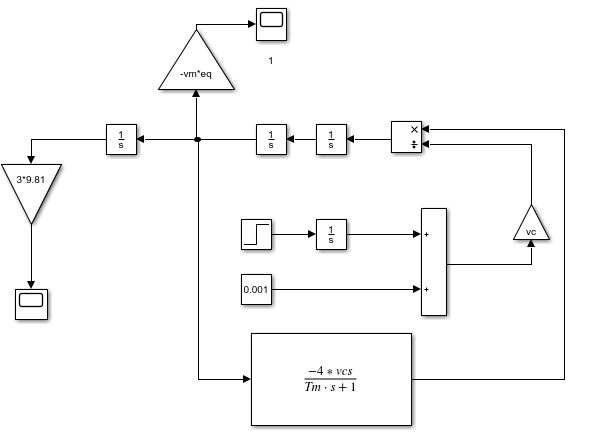
\includegraphics[scale= 0.7]{simAdj.JPG}
    \caption{Simulink dijagram adjungovanog sistema}
    \label{fig:simAdj}
\end{figure}
Simulacija za date vrijednosti daje promašaj usljed početne greške nišanjenja i 
promašaj usljed konstantnog manevra mete i oni su prikazani na slici \ref{fig:adjDet}.
\begin{figure}[!ht]
    \centering
    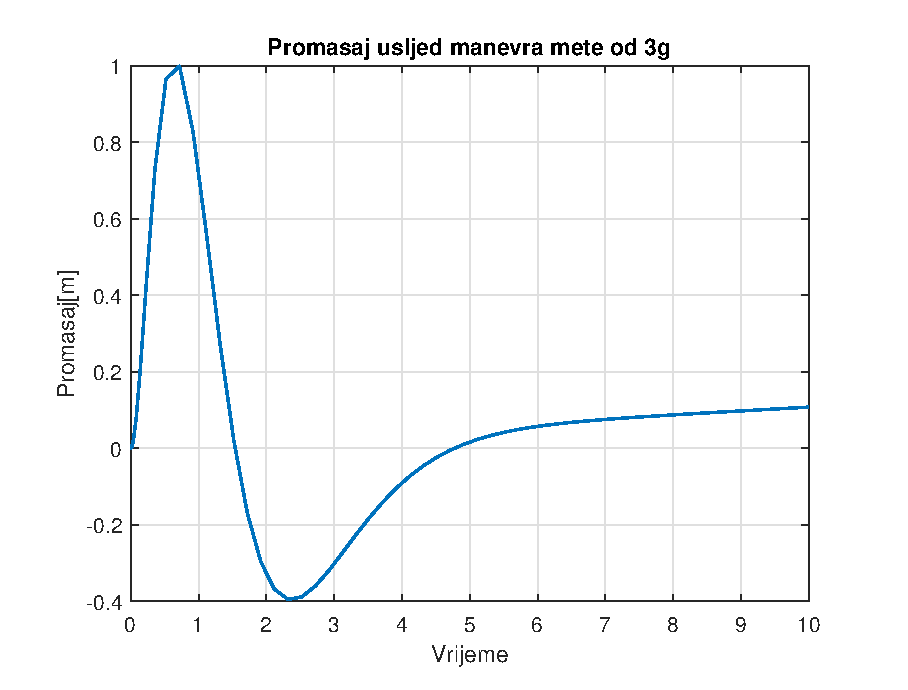
\includegraphics[scale=0.5]{missAdjDet.eps}
    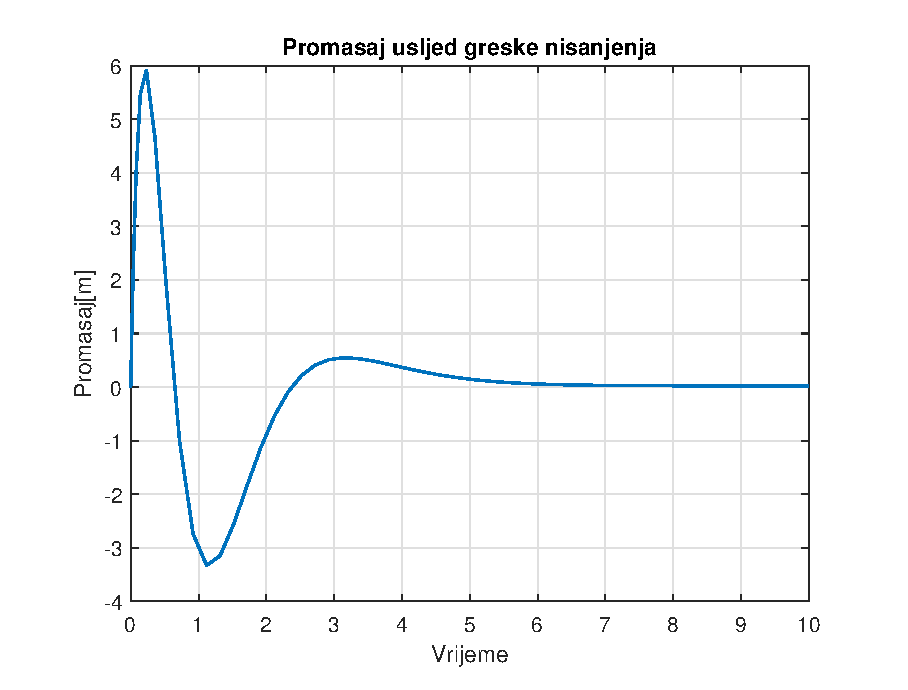
\includegraphics[scale=0.5]{missHead.eps}
    \caption{Odzivi adjungovanog sistema}
    \label{fig:adjDet}
\end{figure}
\section{Adjungovani stohastički sistemi}
Pored mnoštva informacija koje adjungovani sistem daje pri analizi determinističkih 
sistema, adjugnovana tehnika je dosta korisna pri analizi stohastičkih sistema što je 
naročito korisno pri analizi petlje navođenja jer su manevri mete u stvarnosti stohastički. 
Prije nego se prikaže upotreba adjungovane tehnike na petlji navođenja sa stohastičkim 
ulazima, potrebno je se prisjetiti nekoliko važnih definicija.\\
Očekivana vrijednost slučajne promjenljive $x$ čija funkcija gustoće vjerovatnoće $p(x)$ je definisana sa:
\begin{equation}
    E(x)=\int_{-\infty}^{\infty}xp(x)dx
\end{equation}
Standardna devijacija je data sa:
\begin{equation}
    \sigma = \sqrt{E(x^2)-E^2(x)}
\end{equation}
Autokorelaciona funkcija je data sa>
\begin{equation}
    \phi_{xx}(t_1,t_2)=E[x(t_1)x(t_2)]
\end{equation}
Autokorelaciona funkcija predstavlja sličnost dvaju identičnih funkcija 
pri čemu su one smaknute za neki vremenski interval.
Fourieova transformacija autokorelacione funkcije se zove \textit{spektralna 
gustoća snage} i data je sa:
\begin{equation}
    \Phi_{xx}=\int_{-\infty}^{\infty}\phi_{xx}(\tau)e^{-j\omega\tau}d\tau
\end{equation}
Kod bijelog šuma spektralna gustoća snage je konstanta tj.
\begin{equation}
    \Phi_{xx}=\phi_{0}
\end{equation}
Autokorelaciona funkcija bijelog šuma je delta impuls tj. 
\begin{equation}
    \phi_{xx}=\Phi_{0}\delta(t)
\end{equation}
Ovo znači da je bijeli šum samo u jednoj tački identičan samom sebi. 
Kod stohastičkih sistema, izlaz je opisan očekivanom vrijednosšću kvadrata izlaza. 
Prema tome, ako su ulazi tipa bijelog šuma tada vrijedi:
\begin{equation}
    y^2(t)=\int_{-\infty}^tx(\tau_1)h(t,\tau_1)d\tau_1\int_{-\infty}^tx(\tau_2)h(t,\tau_2)d\tau_2
\end{equation}
Ako je $x(t)$ slučajna promjenljiva, može se naći i očekvana vrijednost kvadrata izlaza:
\begin{equation}
    E[y^2(t)]=\int_{-\infty}^t\int_{-\infty}^th(t,\tau_1)h(t,\tau_2)E[x(\tau_1)x(\tau_2)]d\tau_1d\tau_2
\end{equation}
Ako je ulaz $x(t)$ tipa bijelog šuma spektralne gustoće snage $\Phi$, tada se prethodni 
dovjni integral može pojednostaviti zbog impuslne prirode autokorelacione funkcije 
bijelog šuma, pa vrijedi:
\begin{equation}
    E[y^2(t)]=\Phi \int_{-\infty}^t h^2(t,\tau)d\tau
\end{equation}
Sada se prisjetimo da je impulsni odziv adjungovanog sistema $h^*(t_f-\tau,t_f-t)=h(t,\tau)$
 i nakon uvođenja smjene $x=t_f-\tau$, dobija se:
\begin{equation}
    E[y^2(t)]=\Phi\int_{t_f-t}^{t_f}[h^*(x,t_f-t)]^2dx
\end{equation}
Pošto je u interesu promašaj na kraju leta, to je:
\begin{equation}
    E[y^2(t_f)]=\Phi\int_{0}^{t_f}[h^*(x,0)]^2dx
\end{equation}
Sada se vidi da se očekivana vrijednost kvadrata izlaza može dobiti tako što se 
kvadrira i integrira izlaz stohstičkog sistema i to sve u toku samo jedne simulacije. 
Prednost adjungovane metode postaje veća kada se uzme u obzir da na stohastički sistem 
može djelovati više slučajnih ulaza. Kod adjungovane metode, ulazi postaju izlazi pa se 
superpozicijom pri samo jednoj simulaciji može dobiti tačna statisička analiza stohastičkog sistema i 
analiza utjecaja svakog ulaza(tipa bijelog šuma) na performanse sistema. \\
Sada pretpostavimo da meta izvodi manevar konstantnog normalnog ubrazanja i da ga 
počinje izvoditi u trenutku $T$ koji je dat uniformnom raspodjelom i to tako da vrijedi:
\begin{equation}
    p(t)=
    \begin{cases}
        \frac{1}{t_f}, \quad za 0\leq t\leq t_f\\
        0 \qquad za t\geq T\\
    \end{cases}
\end{equation}
Prema tome ulaz u petlju vođenja je dat sa:
\begin{equation}
    x(t)=n_Tu(t-T)
\end{equation}
Ovo znači da je vjerovatnoća pojave manevra jednako vjerovatno u toku cijelog leta. 
Prema tome, autokorelaciona funkcija ulaza u petlju vođenja je:
\begin{equation}
    \phi_{xx}(t_1,t_2)=\int_{-\infty}^{\infty}x(t_1)x(t_1)p(T)dT
\end{equation}
pa se dobija:
\begin{equation}
    \phi_{xx}(t_1,t_2)=\int_{0}^{t_f}n_T(t_1-T)n_T(t_2-T)\frac{dT}{t_f}
\end{equation}
Ako se pretpostavi da je $0<t_1<t_2<t_f$, dobija se autokorelacione funkcija ulaza:
\begin{equation}
    \phi_{xx}(t_1,t_2)=\frac{n_T^2}{t_f}\int_{0}{t_1}dT
    \label{eq:autoCorrxx}
\end{equation}
Autokorelaciona funkcija sistema sa impulsnim odzivom $h(t)$ koji je vođen bijelim 
šumom se može izraziti kao:
\begin{equation}
    \phi_yy(t_1,t_2)=\int_{-\infty}^{t_1}h(t_1-\tau)\int_{-\infty}^{t_2}h(t_2-\tau)\phi_{uu}(\tau_1,\tau_2)d\tau_1d\tau_2
\end{equation}
Gdje je $\phi_{uu}(t_1,t_2)= \Phi_u\delta(\tau_1-\tau_2)$, autokorealciona funkcija bijelog šuma
i $\Phi_u$ je spektralna gustoće snage i pretpostavlja se da je ona konstantna za cijelo vrijeme leta tj. da vrijedi:
\begin{equation}
    \Phi_u(t) = \begin{cases}
        \Phi_u, \quad 0 \leq t \leq t_f \\
        0, \quad \text{inače} 
    \end{cases}
\end{equation}
Pa se dobija:
\begin{equation}
    \phi_yy(t_1,t_2) = \Phi_u\int_0^{t_1}h(t_1-\tau)h(t_2-\tau)d\tau1
\end{equation}
Sada poredeći prethodnu jednačinu sa \ref{eq:autoCorrxx} zaključuje se da 
su dvije autokorelacione funkcije iste ako je: 
\begin{eqnarray}
    \Phi_u =\frac{n_T^2}{t_f} \\
    h(t)=1
\end{eqnarray}
Sada se vidi da je manevar konstante amplitude $n_T$, kod koga je vrijeme 
početka djelovanja uniformno raspoređeno u toku vremena leta $t_f$ ima istu 
autokorelacionu funkciju kao i linearni sistem sa prenosnom funkcijom $H(s)=\frac{1}{s}$ 
na koji djeluje bijeli šum spektralne gustoće snage dat sa: 
\begin{equation*}
    \Phi_u(t) = \begin{cases}
        \Phi_u, \quad 0 \leq t \leq t_f \\
        0, \quad \text{inače}
    \end{cases}
\end{equation*}
Sada će se prikazati primjena adjungovane tehnike na sthastički sistem. Važe ista pravila 
za kreiranje adjungovanog sitema kao i ranije sa jednim dodatnim pravilom da se 
svi stohastički ulazi se moraju modelirati kao bijeli šum koji na kraju postaju 
izlazi adjungovanog sistema. Pošto se ulaz originalnog sistema modelira kao bjeli šum 
kroz integrato, adjungovani model će promjeniti tok signala i kvadrirati i integrisati izlaz.
Dobijeni adjungovani model je prikazan na slici \ref{fig:adjStohastic}.
\begin{figure}[!ht]
    \centering

    \begin{tikzpicture}[auto, node distance=2cm,>=latex']
        \node[block] (nt) {$\frac{1}{s}$};
        \node[block, right of = nt](int1){$\frac{1}{s}$};
        \node[right of = int1] (center){};
        \node[block, right of = center](int2){$\frac{1}{s^2}$};
        \node[sum, right of = int2, node distance = 2cm](sum){+};
        \node[block, right of = sum](div){$\frac{1}{v_{cl}t}$};
        \node[block, below of = int2](law){$-\frac{N'v_{cl}s}{1+sT_m}$};
        \node[name = delta, above of = sum, node distance = 1.5cm](delta){$\delta(0)$};
        \node[left of = nt](out){};
        \node[right of = div](a){};
        \node[left of = nt, node distance = 1.5cm](b){};
       \node[block, below of = b, node distance = 1cm](sq){$()^2$};
       \node[block,below of = sq, node distance = 1.5cm](ro){$\frac{1}{s}$};
       \node[block,right of = ro](gain){$\frac{n_T^2}{t}$};
       \node[right of = gain](out1){$E\left[y^2(t_f)\right]$};
       \draw[->](gain)--(out1);
       \draw[->](ro)--(gain);
       \draw[->](sq)--(ro);
       \draw[->](nt)-|(sq);
        \draw[->](delta)--(sum);
        \draw[->](sum)--(int2);
        \draw[->](int1)--(nt);
        \draw[->](div)--(sum);
        \draw[->](int2)--(int1);
        \draw[->](center.south)-- ++(0,0.13)|-(law);
        \draw[-](law)-|(a.east) -- ++(0,0.0215);
        \draw[->](a.east)-- ++(0.0215,0)--(div);
        \end{tikzpicture}
    \caption{Adjungovani stohastički model}
    \label{fig:adjStohastic}
\end{figure}
Na slici \ref{fig:adjStohasticSimm} je prikazan Simulink model ajdungovanog stohastičkog sistema. 
Impulsni signal je u Simulink modelu unešen kao početni uslov na odgovarajućem integratoru. 
\begin{figure}[!ht]
    \centering
    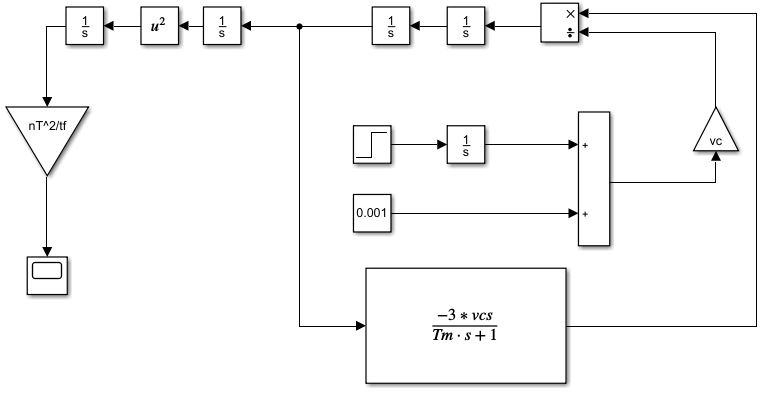
\includegraphics[scale=0.5]{adjStohastic.JPG}
    \caption{Simulink model ajdungovanog stohastičkog sistema}
    \label{fig:adjStohasticSimm}
\end{figure}
Dobija se očekivana vrijednost kvadrata promašaja kao što je prikazano na grafiku \ref{fig:stohGraf}
\begin{figure}[!ht]
    \centering
    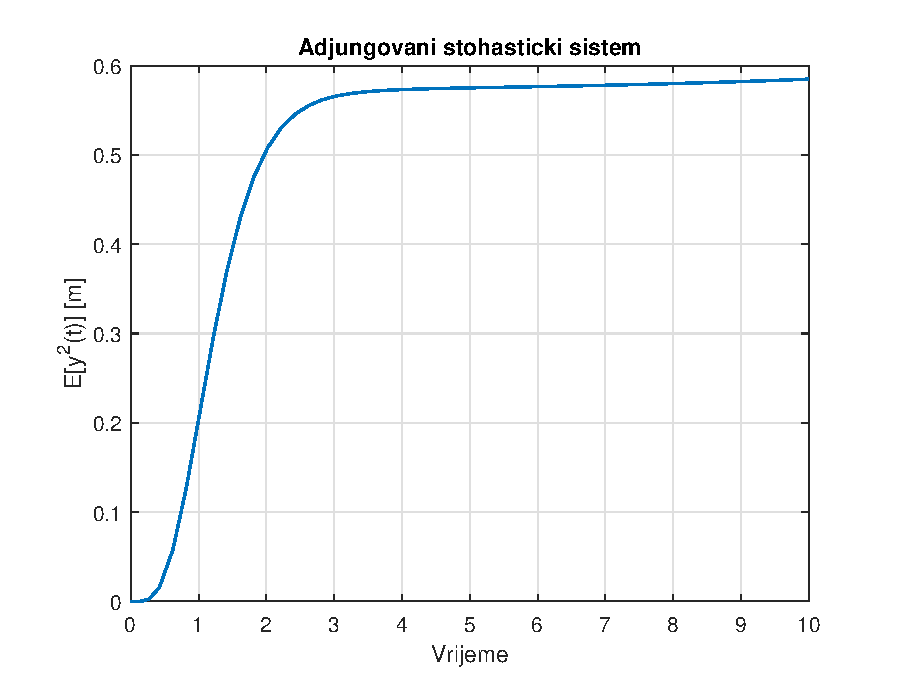
\includegraphics[scale=0.5]{adjStohasticSim.eps}
    \caption{Očekivana vrijednost kvadrata promašaja}
    \label{fig:stohGraf}
\end{figure}
Vidi se da je očekivana vrijednost kvadrata promašaja naglo porasla u prve tri sekunde leta. 
Ovo je zbog toga što je upravo u tom intervalu promašaj najveći, nakon toga promašaj počinje opadati.





\chapter{Sinteza autopilota}
Autopilot je sistem sa zatvorenom povratnom spregom unutar sistema za vođenje objekta 
u prostoru koji osigurava da projektil dostigne ubrzanje koje mu sistem vođenja zapovjeda. 
Funkcija autopilota je da stabilizuje i vodi projektil tako što zadaje upravljačke signale kontrolnim 
površinama koji tjeraju projkeil da se rotira ondnosno da translira.  
Pošto tranzijentni odziv projektila varira sa promjenom uslova leta, tako i parametri 
autopilota treba da se mjenjaju sa uslovima leta pa prema tome dobro 
dizajniran autopilot osigurava skoro linearan odziv. Najčešće se za projektovanje 
autopilota koristi linerizirani model drugog reda koji je ranije izveden. 
\section{Upravljanje i stabilizacija ugla propinjanja}
Glavni zadatak autopilota ugla propinjanja je da stabilizuje projektil, tj. da 
da pruži stabilizaciju propinjanja projektila oko longitudinalne ose. Ovo se postiže tako 
što se mjeri brzina propinjnanja i taj signal se koristi da bi se otklonile 
kontrolne površine za iznos koji je potreban da bi se borilo protiv poremećaja. 
Poremećaji u uglu propinjanja mogu nastati zbog atmosferskih porejemćaja ili 
zbog asimetričnosti letjelice. Dalje, često se zahtjeva da ugao propinjanja prati 
određenu referentnu vrijednost. Ovo se može zahtjevati kod "zemlja- zrak" projektila 
kod kojih se zahtjeva da projektil ima isti ugao pri kojem je lansiran sa platforme. 
Viđeno je ranije da odziv ugla propinjanja neograničeno raste na stalan otklon krmila visine 
i da u početku leta ima kratkoperiodične oscilacije. Uvođenjem povratne sprege,
može se postići da ugao propinjanja postigne zadatu stacionarnu vrijednost, ali kratkoperiodične 
oscilacije će i dalje ostati i mogu praviti probleme. Kratkoperiodične 
oscilacije se mogu uklnoiti uvođenjem dodatne povratne sprege po brzini ugla propinjanja 
i time povećati stabilnost procesa. Uvođenjem intgeralnog kompenzatora može se povećati brzina odziva.
U nastavku će se projektovati regulator ugla propinjanja za linerizirani model longitudinalnog kretanja 
koji je dat prenosnom funkcijom:
\begin{equation}
    \frac{\Delta \theta(s)}{\Delta \delta_V(s)}=\frac{K(T_1s+1)}{s(T^2s^2+2\xi Ts+1)}
\end{equation}
Za $K=0.75$, $T_1 = 1s$, $\omega _n = 20 \frac{rad}{s}$ i $\xi = 0.1$. 
Postojenje nule u prenosnoj funkciji uvodi oscilacije i povećava preskok sistema sa 
zatvorenom povratnom spregom. Odziv ugla propinjanja na odskočnu pobudu  je dat na 
slici \ref{fig:propinj}
\begin{figure}[!ht]
    \centering
    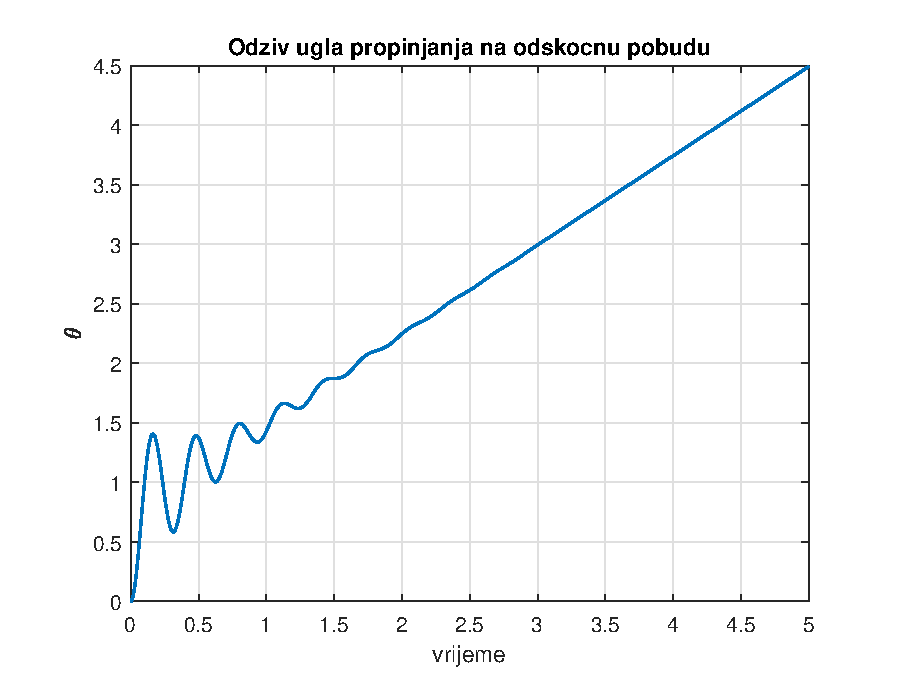
\includegraphics[scale = 0.7]{thetaOtvSprega.eps}
    \caption{Oodziv ugla propinjanja u otvorenoj povratnoj sprezi}
    \label{fig:propinj}
\end{figure} 
Ako se želi da ugao propinjanja prati neku referentnu vrijednost može se uvesti 
povratna sprega po uglu propinjanja preko slobodnog brzinskog žiroskopa. Blok dijagram sistem sa zatvorenom 
povratnom spregom po uglu propinjanja dat je na slici \ref{fig:slobGyro}.
 \begin{figure}[!ht]
     \centering
     \begin{tikzpicture}[auto, node distance=2cm,>=latex']
       \node[input, name=input](input){};
       \node[sum, right of = input](sum){};
       \node[block, right of = sum] (g1){$\frac{K(T_1s+1)}{T^2s^2+2\xi Ts+)}$};
       \node[block, right of = g1,node distance = 2.5cm] (g2){$\frac{1}{s}$};
       \node [output, right of = g2] (output) {};
       \node[block, below of = g1] (gyro){$K_G$};
       \draw [->] (g2) -- node [name=y, anchor = south] {$\theta$}(output);
       \draw[->] (y)|-(gyro);
       \draw[->] (gyro) -|node[pos=0.99] {$-$}(sum);
       \draw[->](g1) -- (g2);
       \draw [draw,->] (input) -- node {$u$} node[pos=0.99] {$+$}(sum);
       \node[anchor = south] (thetadot) at ($(g1)!0.6!(g2)$){$\dot{\theta}$};
       \draw[->] (sum)--(g1);
\end{tikzpicture}
\caption{Povratna sprega po uglu propinjanja}
\label{fig:slobGyro}
\end{figure}
Prenosna funkcija sistema sa zatvorenom povratnom spregom je data sa:
\begin{equation}
    \frac{\theta (s)}{\delta _V(s)} = \frac{\frac{K_GK(T_1s+1)}{T^2s^2+2\xi Ts+)}}{1+\frac{K_GK(T_1s+1)}{T^2s^2+2\xi Ts+)}}
    =\frac{K(T_1s+1)}{T^2s^3+2\xi Ts^2+(1+KK_GT_1)s+KK_G}
\end{equation}
Sada se vidi da je stacionarna vrijednost odziva ugla propinjanja na odskočnu pobudu:
\begin{equation}
    \theta _{stac} = \lim_{s \to 0} s\frac{1}{s}\frac{K(T_1s+1)}{T^2s^3+2\xi Ts^2+(1+KK_GT_1)s+KK_G} = \frac{1}{K_G}
\end{equation}
Odziv ugla propinjanja sa zatvorenom povratnom spregom po uglu propinjanja je data na slici \ref{fig:closedPitch}
\begin{figure}[!ht]
    \centering 
    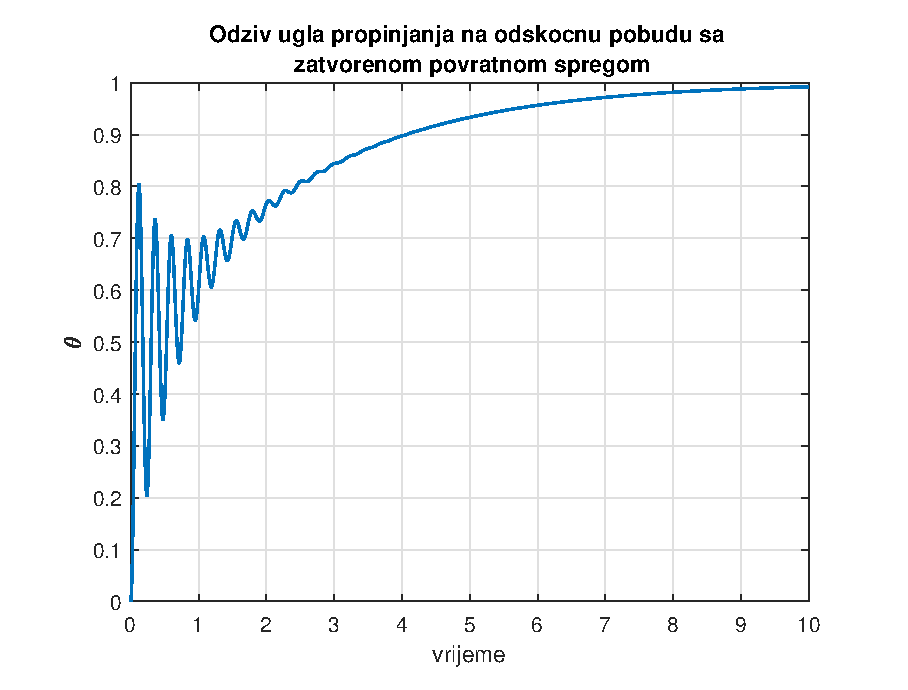
\includegraphics{closedLoopPitch.eps}
    \caption{Odziv ugla propinjanja sa zatvorenom povratnom spregom po uglu propinjanja}
    \label{fig:closedPitch}
\end{figure}
Sada se vidi da se uvođenjem povratne sprege po uglu propinjnja osigurava da ugao propinjanja prati referentnu 
vrijednost, ali se vidi i da je odziv sporiji  i da i dalje postoje kratkoperiodične oscilacije na početku propinjnanja.
Ove oscilacije su posljedica postojanja nule u prenostnoj funkciji zatvorene petlje. 
Uvođenjem integralnog kompenzatora, ova nula se može pokratiti sa polom kompenzatora i tako dobiti glađi odziv.
Uvedimo kompenzator sa prenosnom funkcijom:
\begin{equation}
    G_c(s) = \frac{\alpha T_cs+1}{T_cs+1}  \quad \alpha<1
\end{equation}
Ako se za pol kompenzatora uzme $T_c = T_1$, tada će nula sistema sa otvorenom 
povratnom spregom biti u $-\frac{1}{\alpha T_1}$ što daje veću kontrolu nad postavljanjem 
polova. Povoljnim odabirom parametra $\alpha$ nula se može postaviti na proivoljnu lokaciju.
Odziv sistema sa integralnim kompenzatorom je prikazan na slici \ref{fig:komp}.
\begin{figure}[!ht]
    \centering
    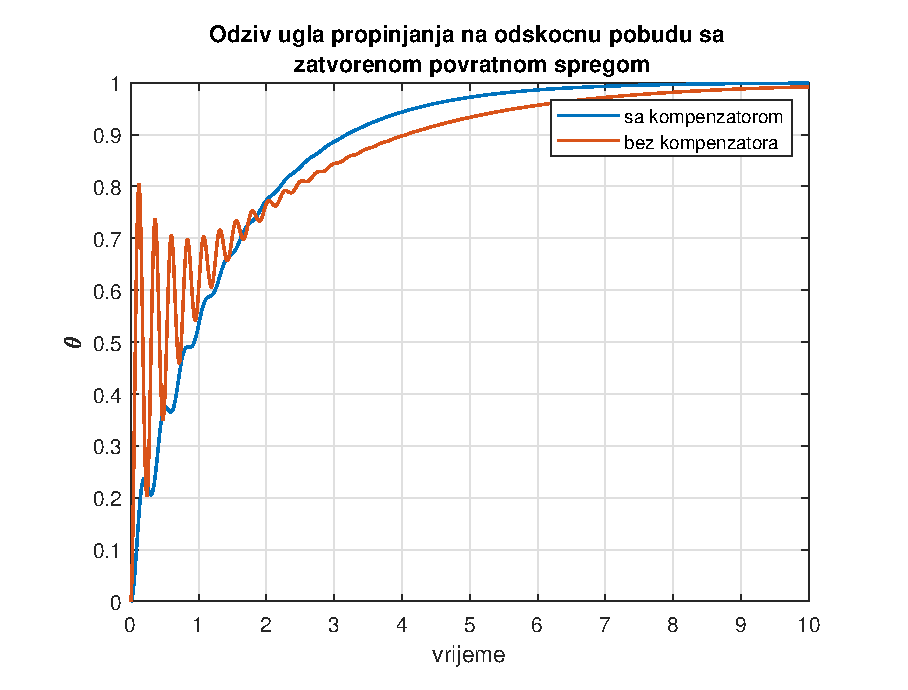
\includegraphics{compareLead.eps}
    \caption{Odziv ugla propinjanja sa integralnim kompenzatorom}
    \label{fig:komp}
\end{figure}
Dodatno, stabilnost odziva se može povećati uvođenjem dodatne povratne sprege po brzini 
ugla propinjanja. Ako se uvede povratna samo po brzini, tada će se stabilizovati samo 
brzina promjene ugla propinjanja a sam ugao propinjanja će imati oblik rampe. 
Blok dijagram ovog upravljačkog sistema je dat na slici \ref{fig:kask}.
\begin{figure}[!ht]
    \centering
    \begin{tikzpicture}[auto, node distance=2cm,>=latex']
        \node[input, name=input](input){};
       \node[sum, right of = input](sum2){};
       \node[sum, right of = sum2](sum){};
       \node[block, right of = sum] (g1){$\frac{K(T_1s+1)}{T^2s^2+2\xi Ts+)}$};
       \node[block, right of = g1,node distance = 2.5cm] (g2){$\frac{1}{s}$};
       \node [output, right of = g2] (output) {};
       \node[block, below of = g1] (gyrosA){$K_{GB}$};
       \node[block, below of = gyrosA, node distance = 1.5cm] (gyro){$K_{GA}$};
       \draw [->] (g2) -- node [name=y, anchor = south] {$\theta$}(output);
       \draw[->] (y)|-(gyro);
       \draw[->] (gyro) -|node[pos=0.99] {$-$}(sum2);
       \draw[->](g1) -- (g2);
       \draw [draw,->] (input) -- node {$u$} node[pos=0.99] {$+$}(sum2);
       \node[anchor = south] (thetadot) at ($(g1)!0.6!(g2)$){$\dot{\theta}$};
       \draw[->] (sum)--(g1);
       \draw[->] (sum2) -- node[pos = 0.99]{$+$}(sum);
       \draw[->] (gyrosA)-| node[pos = 0.99] {$-$}(sum);
       \draw[->] (thetadot)|-(gyrosA);
\end{tikzpicture}
\caption{Povratna sprega po brzini i uglu propinjanja}
\label{fig:kask}
\end{figure}
Vrijednost izvoda ugla propinjanja se dobija pomoću brzinkskog žiroskopa, a 
vrijednost ugla propinjanja se dobija pomoću slobodnog žiroskopa. Pojačanje povratne 
grane iznosi:
\begin{equation}
    H(s)=K_GA+sK_{GB}
\end{equation}
,a pojačanje direktne grane je:
\begin{equation}
    P(s)=\frac{1}{s}\frac{K(T_1s+1)}{T^2s^2+2\xi Ts+)}
\end{equation}
Pa je ukupna funkcija prenosa:
\begin{equation}
    \frac{\theta(s)}{\delta _V(s)} = \frac{K(T_1s+1)}{T^2s^3+
    (2\xi T+KK_{GB}T_1)s^2+(1+KK_{GB}+KK_{GA}T_1)s+KK_{GA}}
\end{equation}
Ovaj sistem je brikazan Simulink blok dijagramomo na slici \ref{fig:simuKask}.
\begin{figure}[!ht]
    \centering
    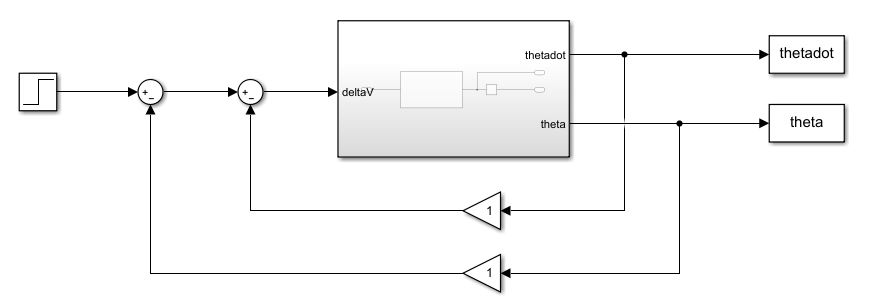
\includegraphics[scale = 0.5]{simKask.JPG}
    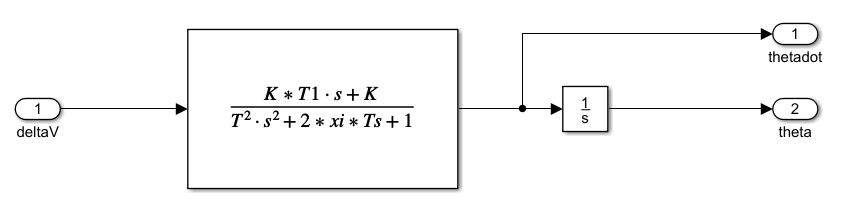
\includegraphics[scale = 0.5]{subKask.JPG}
    \caption{Simulink shema kaskadne regulacije ugla propinjanja}
    \label{fig:simuKask}
\end{figure}
Stacionarna vrijednost na odskočnu pobudu iznosi $\frac{1}{K_{GA}}$
\begin{figure}[!ht]
    \centering
    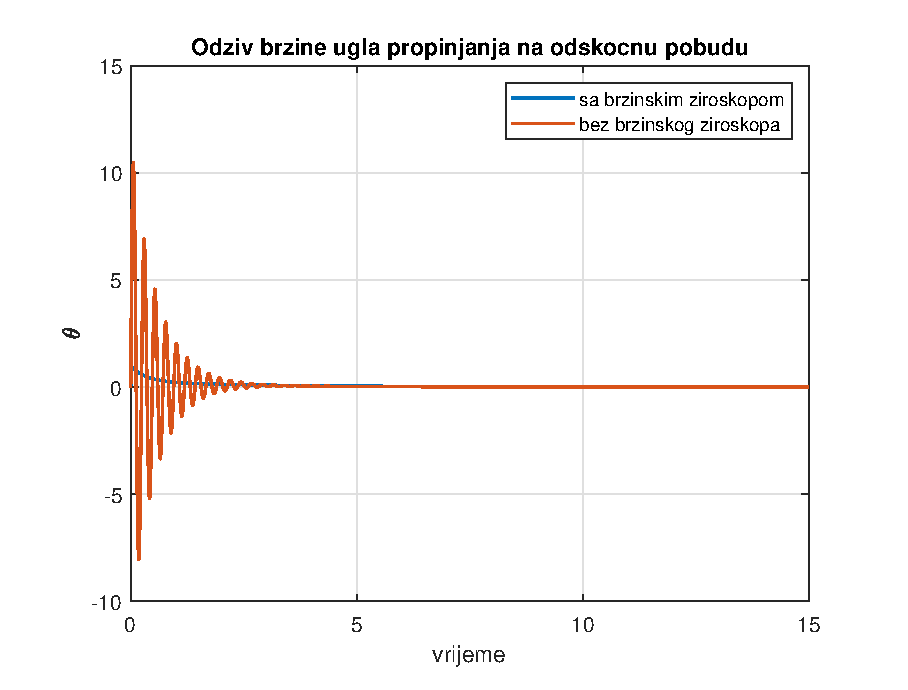
\includegraphics[scale = 0.5]{poredjenjeBrzina.eps}
    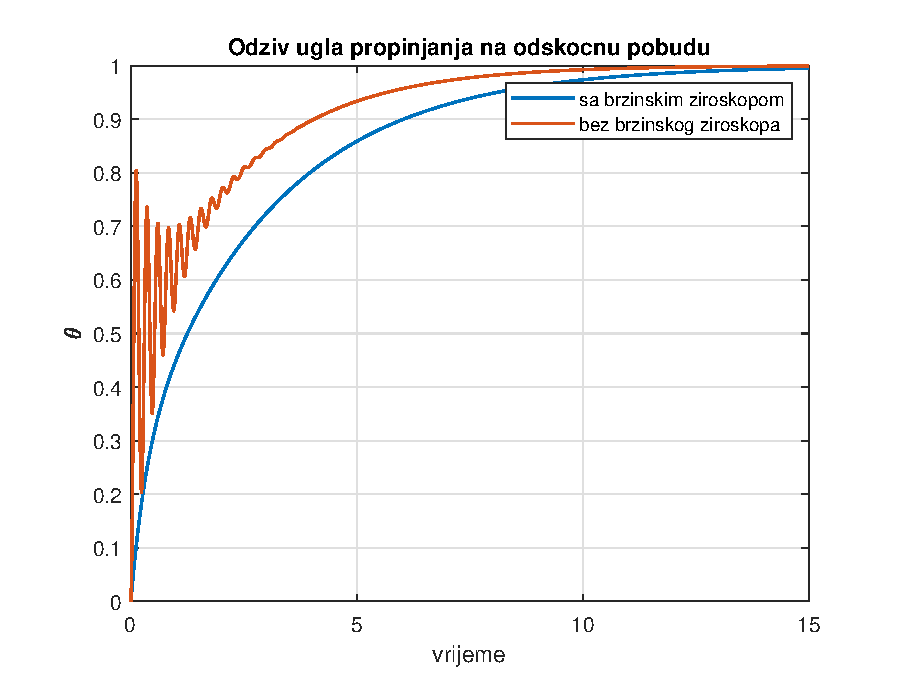
\includegraphics[scale = 0.5]{poredjenjeOdziva.eps}
    \caption{Odzivi ugla propinjanja sa povratnom spregom po brzini i uglu propinjanja}
\end{figure}
%\begin{figure}[!ht]
%    \centering
%    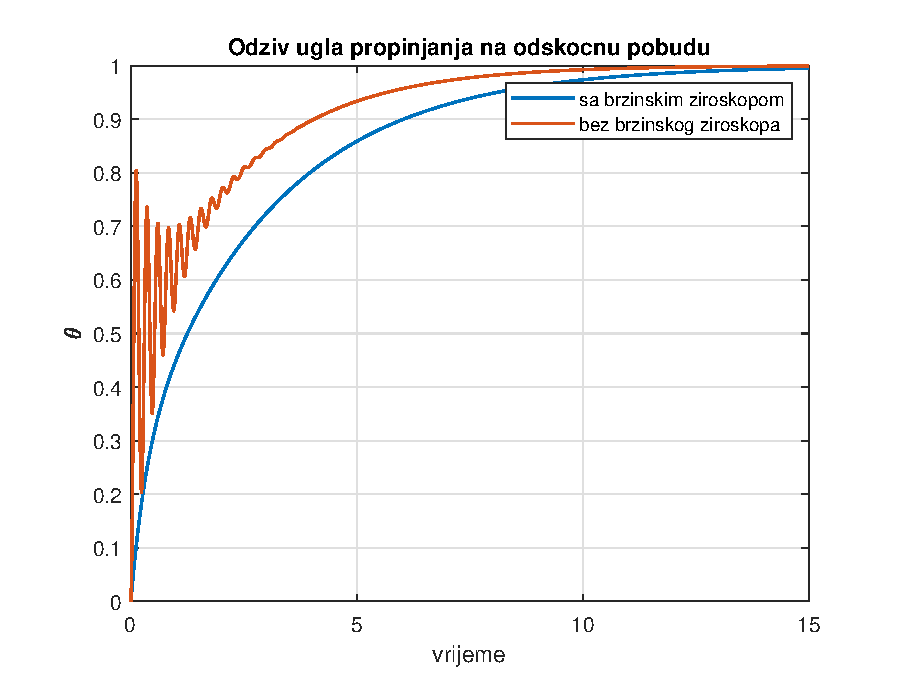
\includegraphics{poredjenjeOdziva.eps}
%\end{figure}
\section{Upravljanje normalnim ubrzanjem}
Kako je razmatrano u prethodnom poglavlju, kod proporcionalne navigacije, se projektilu 
zadaju normalna ubrzanja kako bi on pogodio metu pa je od posebnog interesa imati sitem 
za regulaciju normalnog ubrzanja projektila. Jasno je da će to opet biti upravljanje u 
zatvorenoj povratnoj sprezi. 
\section{Three loop autopilot}
\chapter{Zaključak}
Za razumijevanje problematike vođenja projektila potrebo je više koordinatnih sistema. 
Ostvaren je model projektila sa šest stepeni slobode u koordinatnom sistemu tijela. 
Model projektila se sastoji iz tri nezavisna kanala: kanal visine, kanal pravca i kanal valjanja.
Pokazano je da moguće ostvariti vođenje projektila ka meti regulacijom kanala visine i pravca i 
stabilizacijom kanala valjanja. Za vođenje projektil koristi se zakon proporcionalne navigacije 
koji generiše ubrzanja u referentnom sistemu koji garantuju da će se projektil susresti sa metom.
Prikazan je potpun sistem vođenja zajedno sa autopilotom i pokazano je da 
se ostvaruje pogodak čak i ako postoji razumna početna greška nišanjenja. 


\nocite{*}
\printbibliography

\end{document}